%%%%%%%%%%%%%%%%%%%%%%%%%%%%%%%%%%%%%%%%%
% Imperial College London
% UKRI Centre for Doctoral Training in AI for Healthcare
% https://ai4health.io
%
% LaTeX Template
% Version 1.0 (22/10/19) Aldo Faisal
%%%%%%%%%%%%%%%%%%%%%%%%%%%%%%%%%%%%%%%%%
%----------------------------------------------------------------------------------------
%	PACKAGES AND OTHER DOCUMENT CONFIGURATIONS
%----------------------------------------------------------------------------------------

\documentclass[a4paper,12pt]{article}
\usepackage[french]{babel}
\usepackage[utf8]{inputenc}
\usepackage[T1]{fontenc}
\usepackage{titlesec}
\usepackage{enumitem}
\usepackage{amsmath}
\usepackage{amssymb}
\usepackage{setspace}
\usepackage{fancyhdr}
\usepackage{amsfonts}
\usepackage{graphicx}
\usepackage{array,multirow,makecell}
\usepackage[colorinlistoftodos]{todonotes}
\usepackage[toc,page]{appendix}
\usepackage{geometry}
\usepackage{tocbibind}
 \geometry{
 a4paper,
 total={170mm,257mm},
 left=20mm,
 top=20mm,
 }
 \usepackage{hyperref}
 \hypersetup{
    bookmarks=true,         % show bookmarks bar?
    unicode=false,          % non-Latin characters in Acrobat’s bookmarks
    pdftoolbar=true,        % show Acrobat’s toolbar?
    pdfmenubar=true,        % show Acrobat’s menu?
    pdffitwindow=false,     % window fit to page when opened
    pdfstartview={FitH},    % fits the width of the page to the window
    pdftitle={My title},    % title
    pdfauthor={Author},     % author
    pdfsubject={Subject},   % subject of the document
    pdfcreator={Creator},   % creator of the document
    pdfproducer={Producer}, % producer of the document
    pdfkeywords={keyword1, key2, key3}, % list of keywords
    pdfnewwindow=true,      % links in new PDF window
    colorlinks=false,       % false: boxed links; true: colored links
    linkcolor=red,          % color of internal links (change box color with linkbordercolor)
    citecolor=green,        % color of links to bibliography
    filecolor=magenta,      % color of file links
    urlcolor=cyan           % color of external links
}

\makeatletter
\def\@seccntformat#1{%
  \expandafter\ifx\csname c@#1\endcsname\c@section\else
  \csname the#1\endcsname\quad
  \fi}
\makeatother
\titleformat*{\section}{\center\huge\bfseries}
\titleformat*{\subsection}{\Large\bfseries}
\titleformat*{\subsubsection}{\large\bfseries}
\fancypagestyle{firstpage}{%
  \fancyhf{}%
  \renewcommand{\footrulewidth}{0.1mm}%
  \fancyfoot[R]{ENSIAS}%
  \fancyfoot[C]{\thepage}%
  \fancyfoot[L]{Rapport du projet SI}%
  \renewcommand{\headrulewidth}{0mm}%
}

\thispagestyle{firstpage}


\documentclass{article}

\usepackage{fancyhdr}
\usepackage{float}

\fancypagestyle{firstpage}{%
  \fancyhf{}%
  \renewcommand{\footrulewidth}{0.1mm}%
  \fancyfoot[R]{ENSIAS}%
  \fancyfoot[C]{\thepage}%
  \fancyfoot[L]{Rapport du projet SI}%
  \renewcommand{\headrulewidth}{0mm}%
}  

\fancyhf{}
\renewcommand{\footrulewidth}{0.1mm}
\fancyfoot[R]{ENSIAS}
\fancyfoot[C]{\thepage}
\fancyfoot[L]{Rapport du projet SI}
\fancyhead[L]{\leftmark}


\pagestyle{fancy}


\begin{document}
\begin{titlepage}
\newcommand{\HRule}{\rule{\linewidth}{0.5mm}} % Defines a new command for the horizontal lines, change thickness here
\setlength{\topmargin}{0in}
\center % Center everything on the page
 \begin{center}
\textbf{{UNIVERSITÉ MOHAMMED V }\\ {ÉCOLE NATIONALE SUPÉRIEURE }\\{D'INFORMATIQUE ET D'ANALYSE \\DES SYSTÈMES}\\
{ENSIAS - Rabat}}
\begin{figure}[!h]
\vspace{- 3.3 cm}
\hspace{ 0 cm}

\includegraphics[width=10em]{logo_ensias.jpg}
\end{figure}
\begin{figure}[!h]
\vspace{- 4.8cm}
\hspace{13 cm}

\includegraphics[width=12em]{um5_logo.jpg}
\end{figure}
\end{center}\\[2cm]
%----------------------------------------------------------------------------------------
%	HEADING SECTIONS
%----------------------------------------------------------------------------------------

\textsc{\Large Filière Génie Logiciel (GL) }\\[0.5cm] % Major
\LARGE \textsc{Rapport du projet de l'ingénierie du Web
} \\[1.5cm] 
% Name of your heading such as course name
\textsc{\large }\\[0.5cm] % Minor heading such as course title

%----------------------------------------------------------------------------------------
%	TITLE SECTION
%----------------------------------------------------------------------------------------

\HRule \\[0.4cm]
{ \huge \bfseries Conception et réalisation d'une plateforme de révisison}\\[0.4cm] % Title of your document
\HRule \\[1cm]
 
%----------------------------------------------------------------------------------------
%	AUTHOR SECTION
%----------------------------------------------------------------------------------------
\vspace{1.2cm}
\begin{minipage}{0.4\textwidth}
\begin{flushleft} \large
\emph{Auteurs:}\\
   AARAB\textsc{	Oussama} \\
   AABANE\textsc{	Abderrahim} \\
   ANFAR\textsc{	Asmaa}
   LOUMEDENE\textsc{	Salma}\\
   % Your name, if you are medically qualified please use "Last Name, M.D."
\emph{}

\end{flushleft}
\end{minipage}
\begin{minipage}{0.5\textwidth}
\begin{flushright} \large
\emph{Sous la direction de :} \\
Mr EL HAMLAOUI  \textsc{Mahmoud} 
%\emph{Other Supervisors} \\
% \textsc{Add name here} % Supervisor's Name
% Supervisor Department(s) or NHS Trust+section
\end{flushright}
\end{minipage}\\[5cm]

%----------------------------------------------------------------------------------------
%	DATE SECTION
%----------------------------------------------------------------------------------------
{\large \  Année universitaire : 2020/2021}\\[0.5cm] % Date, change the \today to a set date if you want to be precise

\vfill % Fill the rest of the page with whitespace

\end{titlepage}
%% 100 words
\begin{center}
\centering
    \hspace{4cm}\section*{Remerciements}
\end{center}
\thispagestyle{firstpage}
\onehalfspacing\paragraph{}{Avant de rentrer dans le vif du sujet, nous profitons de l’occasion pour remercier du fond du cœur tous ceux qui ont participé de près ou de loin à la réalisation de cet humble travail. Nos premiers remerciements vont tout d’abord à Mr Mahmoud EL HAMLAOUI qui nous a formé et accompagné tout au long de notre travail avec beaucoup de patience et de pédagogie.

\onehalfspacing\paragraph{}{
Un merci bien particulier adressé également à nos professeurs pour leurs remarques, leurs directives et
l'intérêt qu'ils portent aux étudiants. Nous les remercions sincèrement pour leur suivi et leur orientation.}

\newpage
\tableofcontents
\newpage
\listoffigures

\newpage
\begin{center}
    \section*{\huge\textbf{Introduction générale :}}
\end{center}
\onehalfspacing\paragraph{}{Dans le cadre de sa formation innovante et solide, l'ENSIAS donne l'opportunité à ses élèves ingénieurs de
s'engager dans des projets, favorisant le travail en groupe encadré par des enseignants chercheurs pour qu'ils
puissent développer toute sorte de connaissances acquises en différents langages de programmation.
}
\onehalfspacing\paragraph{}{En deuxième année de notre filière génie logiciel nous sommes appelés à
travailler sur un projet Java EE à travers lequel nous exploitons nos connaisances et compétences acquis durant
notre formation Développement et Ingéniere Web afin d'aboutir à une application Web basé complètement
sur Java EE bien construite.
}
\onehalfspacing\paragraph{}{Le présent document permettra de synthétiser les résultats de ce projet. Ce rapport
sera donc articulé autour de trois grands chapitres : Le premier est consacré au contexte général du projet, le
deuxième chapitre taritera à la partie conception et analyse où nous allons décortiquer le contenu des différents diagrammes des cas d'utilisation
,de séquence et de classe qui concernent notre projet, finalement pour le troisième chapitre nous allons entamer la
réalisation, où nous allons préciser les outils de travail et présenter graphiquement les pages de notre site web à
travers des captures d'écran.
}
\newpage
\vspace*{\stretch{1}}
\begin{center}
		\flushleft\huge\textbf{Chapitre 1}
        \rule{\linewidth}{1mm}
        \flushright\huge\textbf{\section{Contexte général du projet}}
        \thispagestyle{firstpage}
\end{center}
\vspace*{\stretch{1}}
\newpage
\onehalfspacing\paragraph{}{Dans ce chapitre nous allons présenter le contexte général de notre projet ainsi que ses objectifs. Nous aborderons par la suite la méthode adoptée pour le réaliser.}
\subsection{Présentation du projet : }
\onehalfspacing\paragraph{}{Il s’agit d'une application web de gestion des documents des différents éléments de module dédié aux éléves ingénieurs de l'ENSIAS. L'application permet également de créer des Todo listes aidant à la mémorisation des taches qu'un étudiant doit effectuer et qu'il peut visualiser à travers un calendrier réunissant les dates des examens des modules et les taches précisées par cet étudiant.
}
\onehalfspacing\paragraph{}{
Cette application vient pour faciliter la révision à ses utilisateurs en leur assurant un espace de centralisation des ressources de chaque élément (cours, td, tp...), ainsi qu'un meilleure organisation à partir des todo listes.   }
\subsection{Methodologie de travail :}
\onehalfspacing\paragraph{}{ Nous avons choisi comme méthodologie de travail la méthode agile, puisqu’elle est
plus efficace et moins rigide que les méthodes classiques. Elle place les besoins au centre des priorités du projet ce qui offre une plus grande flexibilité et une meilleure visibilité dans la
gestion du projet à partir d’une décomposition de ce dernier en des cycles très courts.
}

\begin{figure}[H]
    \center
    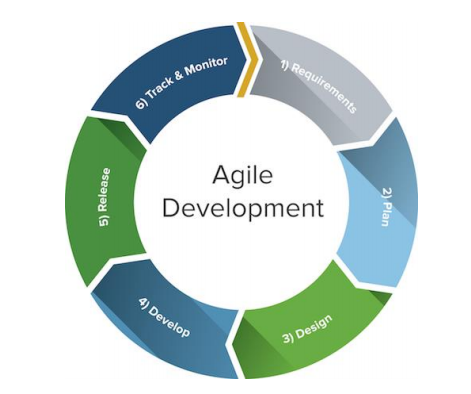
\includegraphics[width=10cm,height=8cm]{agile.png}
    \caption{Cycle Agile}
    \label{fig:Cycle Agile.}
\end{figure}

\vspace{1.8cm}
\subsection{Conclusion  :}
\onehalfspacing\paragraph{}{Le long de cette partie on a présenté le contexte général du projet en introduisant sa description et en précisant ses objectfs.
Dans le chapitre suivant nous allons étudier et analyser le projet et élaborer par la suite la conception du travail.
}
\newpage
\vspace*{\stretch{1}}
\begin{center}
		\flushleft\huge\textbf{Chapitre 2}
        \rule{\linewidth}{1mm}
        \flushright\huge\textbf{\section{Analyse et Conception }}
        \thispagestyle{firstpage}
\end{center}
\vspace*{\stretch{1}}
\newpage
\onehalfspacing\paragraph{}{Cette étape définit généralement les structures et les modèles à suivre lors de la phase d'implémentation de l'application. C'est la phase où nous préparons l'architecture du projet, et où nous définissons la structure
de l'application. Par souci de clarté, nous débuterons par une phase préliminaire où sera présentés les diagrammes des cas d'utilisation. Ensuite, nous poursuivrons par quelques
diagrammes de séquence du système suivis par le diagramme de classe qui illustrera le
processus de fonctionnement du dit système.}
\subsection{Diagramme des cas d'utilisations :}
\onehalfspacing\paragraph{}{Un diagramme de cas d'utilisation capture le comportement d'un système, d'un sous-système, d'une classe ou d'un composant tel qu'un utilisateur extérieur le voit.Les cas d'utilisation permettent d'exprimer le besoin des utilisateurs d'un système, ils sont donc une vision orientée utilisateur de ce besoin au contraire d'une vision informatique.
}

\onehalfspacing\paragraph{}{L'application tient en compte deux acteurs:}

\vspace{0.5cm}
\begin{enumerate}
    \item\textbf{ Utilisateur} :
        \begin{itemize}[label=\textbullet]
        \item S'inscrire
        \item Accéder à un module
        \item Consulter le calendrier
        \item Ajouter une tache dans la Todo liste
        \end{itemize}
    \vspace{0.5cm}
    \item\textbf{ Admin} :
        \begin{itemize}[label=\textbullet]
        \item S'inscrire
        \item Accéder à un module
        \item Consulter le calendrier
        \item Ajouter une tache dans la Todo liste
        \item Créer un module
        \item Modifier un module
        \end{itemize}
\end{enumerate}
\vspace{1.3cm}
\begin{figure}[H]
    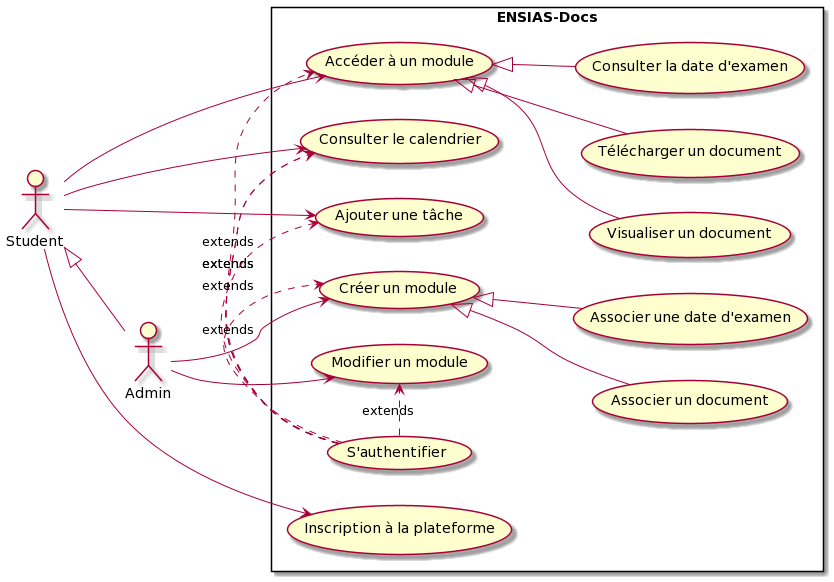
\includegraphics[width=16cm,height=12cm]{JEEUseCase.png}
    \caption{Utilisateur et Admin UC}
    \label{fig:Utilisateur et admin UC.}
\end{figure}


\subsection{Diagramme de séquences :}
\onehalfspacing\paragraph{}{Pour schématiser la vue comportementale de notre système informatique, nous faisons recours au diagramme
de séquence d'UML. Ce diagramme permet de présenter les interactions entre l'acteur et le système avec des
messages présentés dans un ordre chronologique. Ainsi nous établissons :
\vspace{0.2cm}
     \begin{itemize}[label=\textbullet]
        \item Le diagramme de séquence 1: "Accèder à un module"
        \item Le diagramme de séquence 2: "Ajouter un module"
    \end{itemize}
}
\subsubsection{Accèder à un module :}
\begin{itemize}[label=\textbullet]
        \item Description : Ce premier cas d'utilisation permet de chercher dans la liste des modules, en choisir un, et puis visualiser ou télécharger son contenu.
au panier.
        \item Acteur : L'utilisateur de l'application
        \item Pré-conditions : L'utilisateur doit posséder un compte et doit s'authentifier

\end{itemize}
\vspace{5cm}
\begin{figure}[H]
\vspace{2cm}
    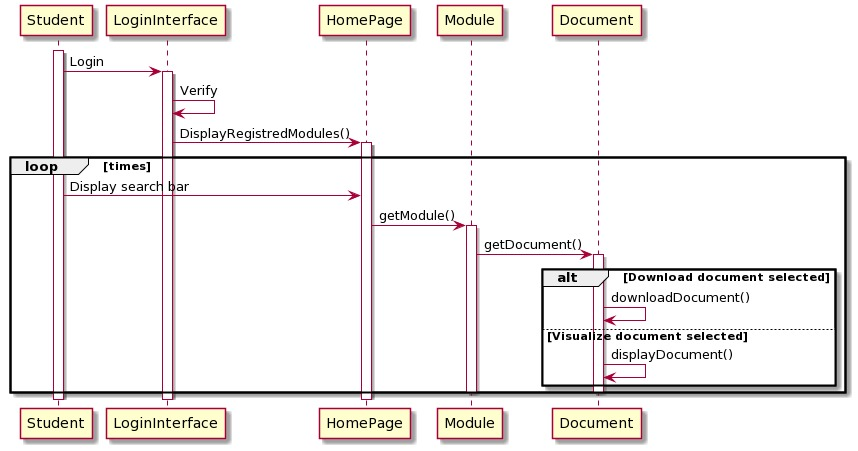
\includegraphics[width=16cm,height=12cm]{seqUser.jpeg}
    \caption{Diagramme de séquences: Accèder à un module}
    \label{fig:Diagramme de séquaneces: Accèder à un module.}
\end{figure}

\vspace{1cm}
\subsubsection{Ajouter à un module :}

\begin{itemize}[label=\textbullet]
        \item Description : Ce deuxième cas d'utilisation permet de chercher d'ajouter un module à l'application.
        \item Acteur : le ou les administrateurs de l'application
        \item Pré-conditions : L'utilisateur doit posséder un compte avec les droit d'administrateur et doit s'authentifier

\end{itemize}
\begin{figure}[H]
\vspace{2cm}
    \center
    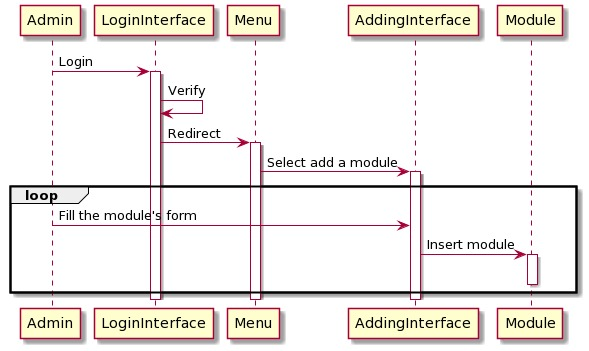
\includegraphics[width=16cm,height=12cm]{seqAdmin.jpeg}
    \caption{Diagramme de séquences: Ajouter un module}
    \label{fig:Diagramme de séquaneces: Ajouter un module.}
\end{figure}

\vspace{1cm}
\subsection{Diagramme d'activité :}
\onehalfspacing\paragraph{}{Les diagrammes d’activités sont considérés comme des diagrammes comportementaux, car ils décrivent ce qui doit arriver dans le système modélisé. Nous allons présenter dans cette partie les deux diagrammes d'activités dont notammennt : "Espace administrateur" et "Espace étudiant".}
\begin{figure}[H]
\vspace{2cm}
    \center
    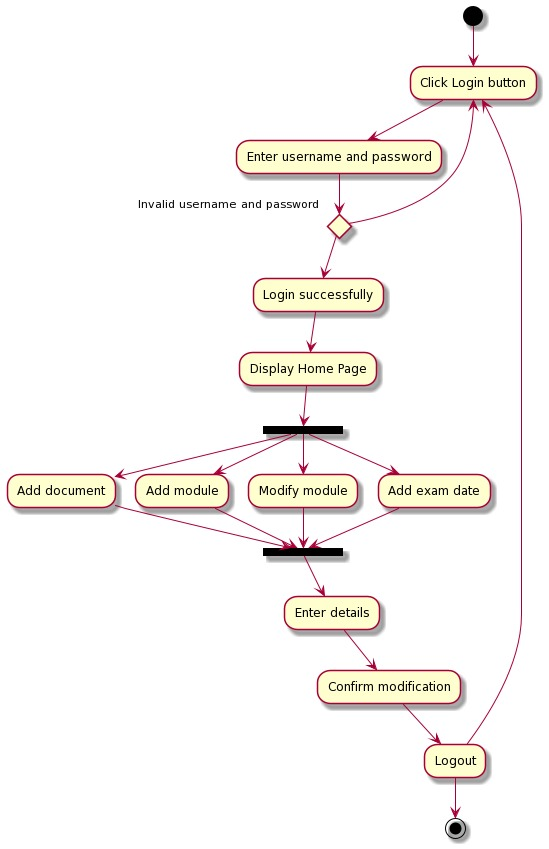
\includegraphics[width=16cm,height=18cm]{small.jpeg}
    \caption{Diagramme d'activité: Espace administrateur}
    \label{fig:Diagramme de séquaneces: Ajouter un module.}
\end{figure}
\begin{figure}[H]

    \center
    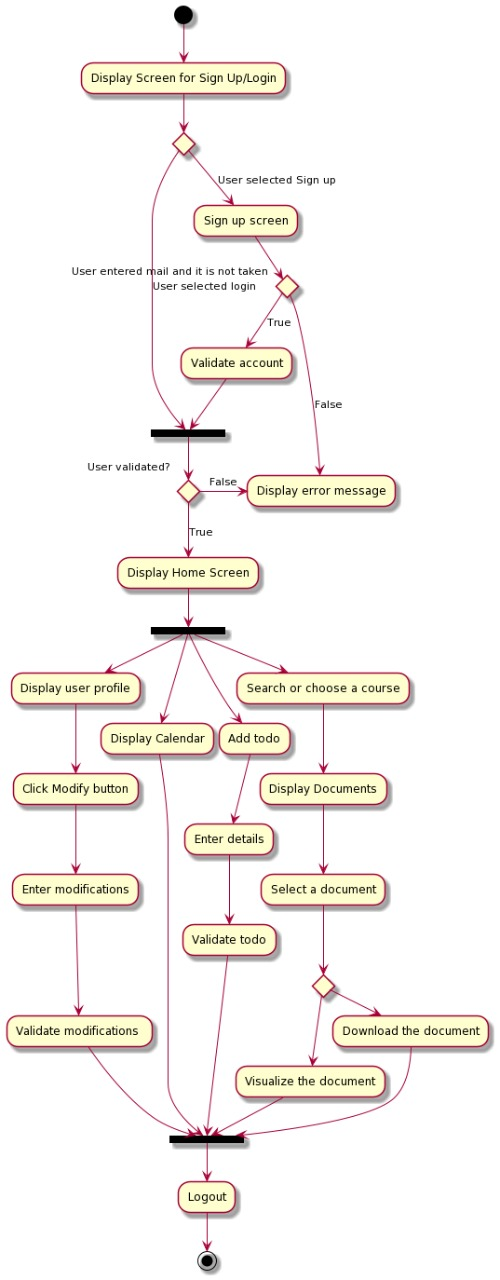
\includegraphics[width=17cm,height=22cm]{big.jpeg}
    \caption{Diagramme d'activité: Espace étudiant}
    \label{fig:Diagramme de séquaneces: Ajouter un module.}
\end{figure}

\vspace{1cm}
\subsection{Diagramme de classes :}
\onehalfspacing\paragraph{}{Ce diagramme consiste à consolider et valider toute l'analyse des cas d'utilisation. Il s'agit d'un regroupement
de l'ensemble des classes en un seul diagramme (diagramme de classe récapitulatif).}

\begin{figure}[H]
    \center
    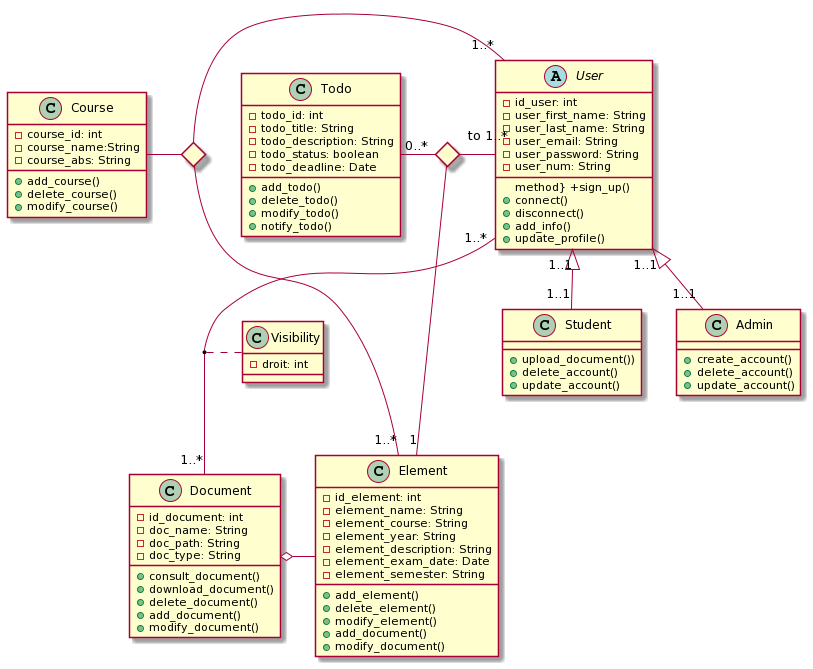
\includegraphics[width=18.3cm,height=16cm]{CLASSDIAGRAM.png}
    \caption{Diagramme de classes}
    \label{fig:Diagramme de classes.}
\end{figure}
\subsection{Conclusion  :}
\onehalfspacing\paragraph{}{Cette partie a été consacrée à l'élaboration des différents diagrammes selon le langage de modélisation unifié
UML: cas d'utilisations, séquences et diagrammes de classes. Ces diagrammes sont nécessaires pour avoir un champ confortable lors de l'implémentation du code de l'application.}


\newpage
\vspace*{\stretch{1}}
\begin{center}
		\flushleft\huge\textbf{Chapitre 3}
        \rule{\linewidth}{1mm}
        \flushright\huge\textbf{\section{Réalisation }}
        \thispagestyle{firstpage}
\end{center}
\vspace*{\stretch{1}}
\newpage

\onehalfspacing\paragraph{}{Dans ce chapitre, nous
entamerons la phase de réalisation qui est l'étape où nous traduisons la conception et les règles par un langage
de programmation afin d'aboutir à une automatisation des fonctionnalités de l'application. Nous allons préciser l'architecture du projet, les outils utilisés et finalement les captures d'écran du résultat final
  .}
\newline
\subsection{Architecture du projet: Pattern MVC}
\onehalfspacing\paragraph{}{Le pattern d'architecture logicielle MVC (Modèle-Vue-Contrôleur) est un modèle destiné à répondre aux
besoins des applications interactives en séparant les problématiques liées aux différents composants au sein de
leur architecture respective. Ce paradigme regroupe les fonctions nécessaires en trois catégories :
}
\vspace{0.5cm}
\begin{itemize}[label=\textbullet]
        \item Un modèle : modèle de données.
        \item Une vue : interface utilisateur.
        \item Un contrôleur : logique de contrôle.
\end{itemize}
\begin{figure}[H]
    \centering
    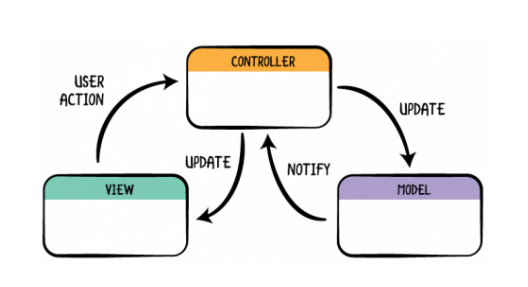
\includegraphics[width=17cm,height=12cm]{mvc.PNG}
    \caption{Design Pattern MVC.}
    \label{fig:Design Pattern MVC.}
\end{figure}
\subsection{Outils de developpement :}
\subsubsection{Langage de programmation: }
\begin{minipage}{0.15\textwidth}
	\begin{minipage}{\linewidth}
		\makebox[\linewidth]{
			
\includegraphics[keepaspectratio=true,scale=0.31,width=5cm,height=3cm]{jee.png}}   
	\end{minipage}
\end{minipage}
\hfill
\begin{minipage}{0.75\textwidth}
\vspace{0.5cm}
	Le terme « Java EE » signifie Java Enterprise Edition. En effet, la plate-forme Java EE est construite sur le langage Java et la plate-forme Java SE, et elle y ajoute un grand nombre de bibliothèques remplissant tout un tas de fonctionnalités que la plate-forme standard ne remplit pas d'origine. L'objectif majeur de Java EE est de faciliter le développement d'applications web robustes et distribuées. [1]\\
\end{minipage}\\

\subsubsection{Outil de gestion de projet: }
\begin{minipage}{0.15\textwidth}
	\begin{minipage}{\linewidth}
		\makebox[\linewidth]{
			
\includegraphics[keepaspectratio=true,scale=0.31,width=4cm,height=3cm]{maven.jpg}}   
	\end{minipage}
\end{minipage}
\hfill
\begin{minipage}{0.75\textwidth}
\vspace{0.5cm}
	Apache Maven (couramment appelé Maven) est un outil de gestion et d'automatisation de production des projets logiciels Java en général et Java EE en particulier. Il est utilisé pour automatiser l'intégration continue lors d'un développement de logiciel. [2]\\
\end{minipage}\\


\subsubsection{Environnement de développement : }
\begin{minipage}{0.15\textwidth}
	\begin{minipage}{\linewidth}
		\makebox[\linewidth]{
			
\includegraphics[keepaspectratio=true,scale=0.31,width=5cm,height=3cm]{eclipse.png}}   
	\end{minipage}
\end{minipage}
\hfill
\begin{minipage}{0.75\textwidth}
\vspace{0.5cm}
	Eclipse IDE est un environnement de développement intégré libre (le terme Eclipse désigne également le projet correspondant, lancé par IBM) extensible, universel et polyvalent, permettant potentiellement de créer des projets de développement mettant en œuvre n'importe quel langage de programmation.\\
\end{minipage}\\

\subsubsection{Gestion de version : }
\begin{minipage}{0.15\textwidth}
	\begin{minipage}{\linewidth}
		\makebox[\linewidth]{
			
\includegraphics[keepaspectratio=true,scale=0.31,width=5cm,height=3cm]{git.png}}   
	\end{minipage}
\end{minipage}
\hfill
\begin{minipage}{0.75\textwidth}
\vspace{0.5cm}
	Git est un système de contrôle de version open-source spécifique créé par Linus Torvalds en 2005.
Concrètement, Git est un système de contrôle de version distribué, ce qui signifie que l’ensemble de la base du code et de l’historique est disponible sur l’ordinateur de chaque développeur, ce qui permet des branchements et une fusion faciles.\\
\end{minipage}\\

\subsubsection{Système de gestion de base de données : }
\begin{minipage}{0.12\textwidth}
	\begin{minipage}{\linewidth}
		\makebox[\linewidth]{
			
\includegraphics[keepaspectratio=true,scale=0.31,width=5cm,height=3cm]{mysql.png}}   
	\end{minipage}
\end{minipage}
\hfill
\begin{minipage}{0.75\textwidth}
\vspace{0.5cm}
	MySQL est un système de gestion de bases de données relationnelles (SGBDR). Il est distribué sous une
double licence GPL et propriétaire. Il fait partie des logiciels de gestion de base de données les plus utilisés
au monde3, autant par le grand public (applications web principalement) que par des professionnels, en
concurrence avec Oracle, Informix et Microsoft SQL Server. [4]
\\
\end{minipage}\\
\subsubsection{Front-end : }
\vspace{0.7cm}
\begin{minipage}{0.12\textwidth}
	\begin{minipage}{\linewidth}
		\makebox[\linewidth]{
			
\includegraphics[keepaspectratio=true,scale=0.31,width=4cm,height=2.2cm]{html.png}}   
	\end{minipage}
\end{minipage}
\hfill
\begin{minipage}{0.75\textwidth}
\vspace{0.5cm}
	L'HyperText Markup Language, généralement abrégé HTML, est le langage de
balisage conçu pour représenter les pages web. C'est un langage permettant d'écrire
de l'hypertexte, d'où son nom.

\\
\vspace{0.7cm}
\end{minipage}\\
\begin{minipage}{0.2\textwidth}
	\begin{minipage}{\linewidth}
		\makebox[\linewidth]{
			
\includegraphics[keepaspectratio=true,scale=0.31,width=4cm,height=2.5cm]{css.png}}   
	\end{minipage}
\end{minipage}
\hfill
\begin{minipage}{0.75\textwidth}
\vspace{0.7cm}
Les feuilles de style en cascade, généralement appelées CSS de l'anglais Cascading
Style Sheets, forment un langage informatique qui décrit la présentation des
documents HTML et XML. Les standards dénissant CSS sont publiés par le World
Wide Web Consortium.


\\
\vspace{0.7cm}
\end{minipage}\\
\begin{minipage}{0.2\textwidth}
	\begin{minipage}{\linewidth}
		\makebox[\linewidth]{
			
\includegraphics[keepaspectratio=true,scale=0.31,width=4cm,height=2.2cm]{js.jpg}}   
	\end{minipage}
\end{minipage}
\hfill
\begin{minipage}{0.75\textwidth}
\vspace{0.7cm}
	JavaScript (qui est souvent abrégé en  JS ) est un langage de script léger, orienté
objet, principalement connu comme le langage de script des pages web.

\vspace{0.7cm}
\end{minipage}\\
\begin{minipage}{0.2\textwidth}
	\begin{minipage}{\linewidth}
		\makebox[\linewidth]{
			
\includegraphics[keepaspectratio=true,scale=0.31,width=2cm,height=2.2cm]{bootstrap.png}}   
	\end{minipage}
\end{minipage}
\hfill
\begin{minipage}{0.75\textwidth}
\vspace{0.7cm}
	Bootstrap est une collection d'outils utile à la création du design (graphisme, animation et interactions
avec la page dans le navigateur ... etc. ...) de sites et d'applications web. C'est un ensemble qui contient
des codes HTML et CSS, des formulaires, boutons, outils de navigation et autres éléments interactifs, ainsi
que des extensions JavaScript en option. [7]
\\
\vspace{0.7cm}
\end{minipage}\\
\begin{minipage}{0.2\textwidth}
	\begin{minipage}{\linewidth}
		\makebox[\linewidth]{
			
\includegraphics[keepaspectratio=true,scale=0.31,width=4cm,height=2.5cm]{jstl.jpg}}   
	\end{minipage}
\end{minipage}
\hfill
\begin{minipage}{0.75\textwidth}
\vspace{0.7cm}
	La JavaServer Pages Standard Tag Library est un composant de la plate-forme JEE
de développement. Elle étend la spécication JSP en ajoutant une bibliothéque de
balises pour les taches courantes, comme le travail sur des chiers XML, l'exécution
conditionnelle, les boucles et l'internationalisation.
\\
\end{minipage}\\

\subsubsection{Serveur de l'application : }
\begin{minipage}{0.15\textwidth}
	\begin{minipage}{\linewidth}
		\makebox[\linewidth]{
			
\includegraphics[keepaspectratio=true,scale=0.31,width=4.5cm,height=2cm]{tomcatt.png}}   
	\end{minipage}
\end{minipage}
\hfill
\begin{minipage}{0.75\textwidth}
\vspace{0.5cm}
Tomcat est un conteneur web libre de servlets et JSP. Issu du projet Jakarta, c'est
un des nombreux projets de l'Apache Software Foundation. [3]\\
\end{minipage}\\

\subsubsection{Outils de test : }
\begin{minipage}{0.15\textwidth}
	\begin{minipage}{\linewidth}
		\makebox[\linewidth]{
			
\includegraphics[keepaspectratio=true,scale=0.31,width=4.5cm,height=3cm]{junit.png}}   
	\end{minipage}
\end{minipage}
\hfill
\begin{minipage}{0.75\textwidth}
\vspace{0.5cm}
JUnit est un framework mature pour permettre l'écriture et l'exécution de tests automatisés unitaires. Les classes de tests JUnit 5 sont similaires à celles de JUnit 4. Cependant, JUnit 5 est une réécriture complète de l'API contenue dans des packages différents de ceux de JUnit 4. [5]\\
\end{minipage}\\
\vspace{0.7}
\begin{minipage}{0.2\textwidth}
	\begin{minipage}{\linewidth}
		\makebox[\linewidth]{
			
\includegraphics[keepaspectratio=true,scale=0.31,width=4cm,height=2.5cm]{arquillian.jpg}}   
	\end{minipage}
\end{minipage}
\hfill
\begin{minipage}{0.75\textwidth}
\vspace{0.7cm}
	Dans un test d’intégration avec Arquillien , le code de test n’est pas dépendant du serveur ! Le code créer dynamiquement une archive et la déploie dans un conteneur cible en fonction de l’adaptateur de conteneur disponible dans le classpath de test.
\\
\end{minipage}\\

\subsubsection{Outil de virstualisation : }
\begin{minipage}{0.15\textwidth}
	\begin{minipage}{\linewidth}
		\makebox[\linewidth]{
			
\includegraphics[keepaspectratio=true,scale=0.31,width=5cm,height=2.5cm]{docker.png}}   
	\end{minipage}
\end{minipage}
\hfill
\begin{minipage}{0.75\textwidth}
\vspace{0.5cm}
Docker permet d’embarquer une application dans un container virtuel qui pourra s’exécuter sur n’importe quelle machine.Disponibles pour les applications Linux et Windows, les “logiciels conteneurisés” fonctionneront toujours de la même façon, quel que soit l’environnement. Les conteneurs isolent le logiciel de son environnement. [6]\\
\end{minipage}\\

\vspace{5cm}
\subsubsection{Plateforme de déploiement : }
\begin{minipage}{0.15\textwidth}
	\begin{minipage}{\linewidth}
		\makebox[\linewidth]{
			
\includegraphics[keepaspectratio=true,scale=0.31,width=2.5cm,height=2.5cm]{aws.png}}   
	\end{minipage}
\end{minipage}
\hfill
\begin{minipage}{0.75\textwidth}
\vspace{0.5cm}
Amazon Web Services (AWS) est la plateforme cloud la plus complète et la plus largement adoptée au monde. Elle propose plus de 200 services complets issus de centres de données du monde entier. Des millions de clients y compris de très grandes entreprises et des agences fédérales de premier plan utilisent AWS pour réduire leurs coûts, gagner en agilité et innover plus rapidement. [6]\\
\end{minipage}\\

\vspace{1.2cm}
\subsection{Présentation de l'application :}
\onehalfspacing\paragraph{}{
Cette partie dénombre la présentation des Scénarios applicatifs de l'application. Nous allons présenter dans
ce qui suit, les imprimes-écran des principales interfaces réalisées dans notre site web.
}
\vspace{15cm}
\subsubsection{Page d'accueil}{C'est la page d'accueil qui s'affiche dès l'accès à notre application web. Elle contient deux options: se connecter ou s'inscrire.
}
\vspace{0.3cm}
\begin{figure}[H]
    \centering
    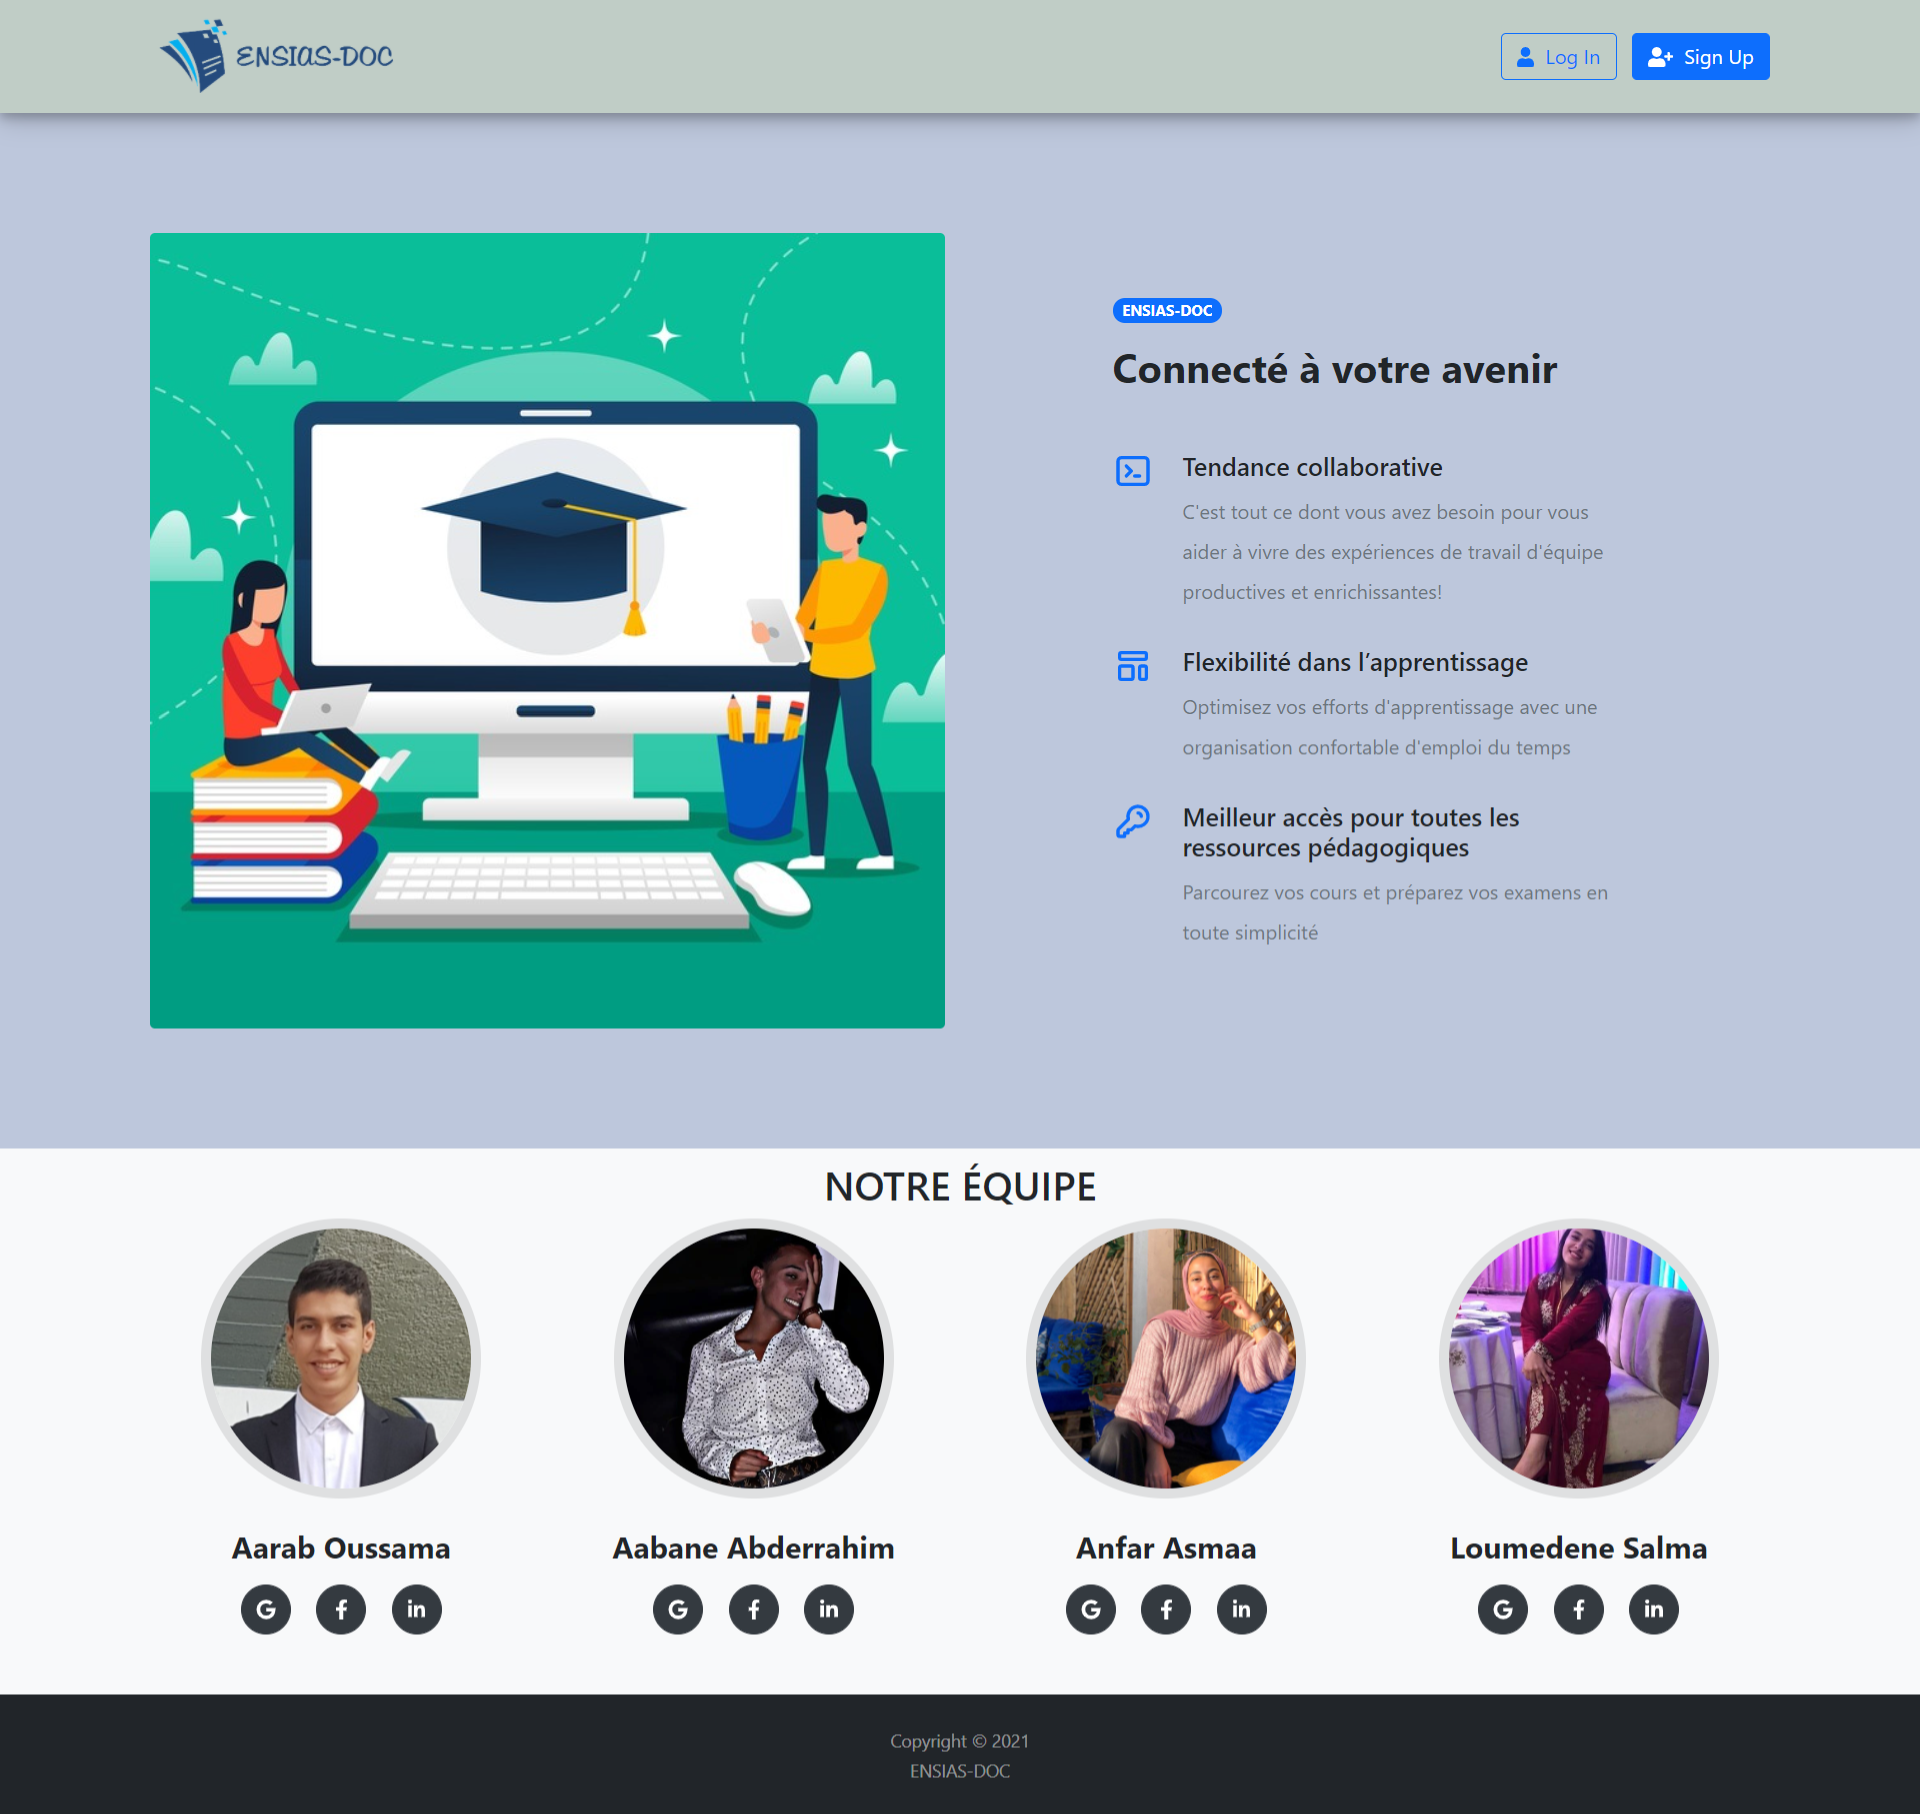
\includegraphics[width=17cm,height=15cm]{index.png}
    \caption{Page d'accueil.}
    \label{Page d'accueil.}
\end{figure}
\vspace{0.3cm}
\subsubsection{Page d'inscription}{Comme dans toutes les plateformes en ligne, le visiteur ne peut profiter des activités qu'après la phase d'inscription, notre application web met à la disposition de ses visiteurs un formulaire d'inscription.
}
\begin{figure}[H]
    \centering
    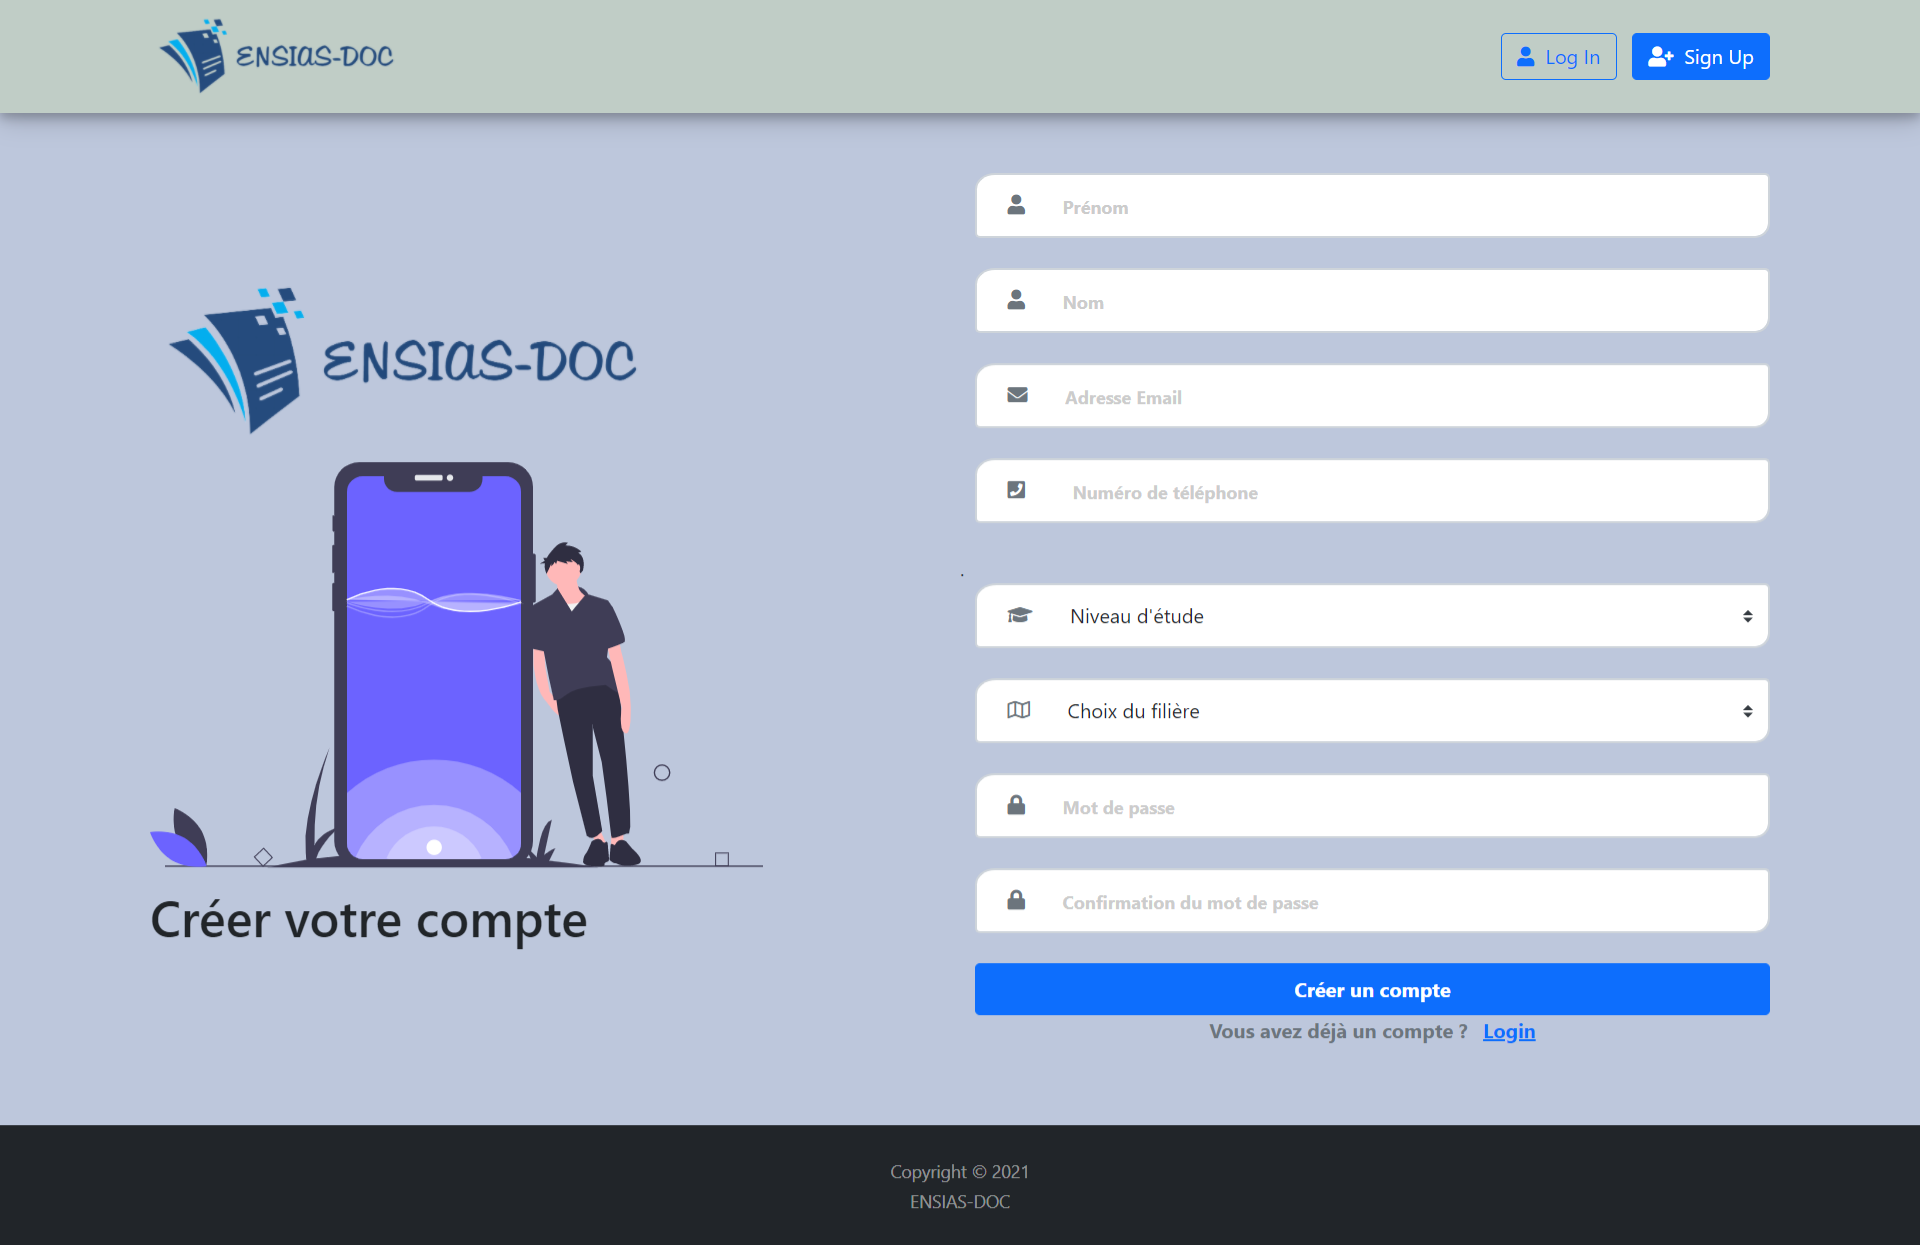
\includegraphics[width=17cm,height=9cm]{enregistrement.png}
    \caption{Page d'inscription.}
    \label{Page d'inscription.}
\end{figure}
\subsubsection{Page d'authentification}{Après la phase d'inscription présentée dans la figure précédante l'utilisateur doit s'authentifier pour avoir accès à son compte.
}

\begin{figure}[H]
    \centering
    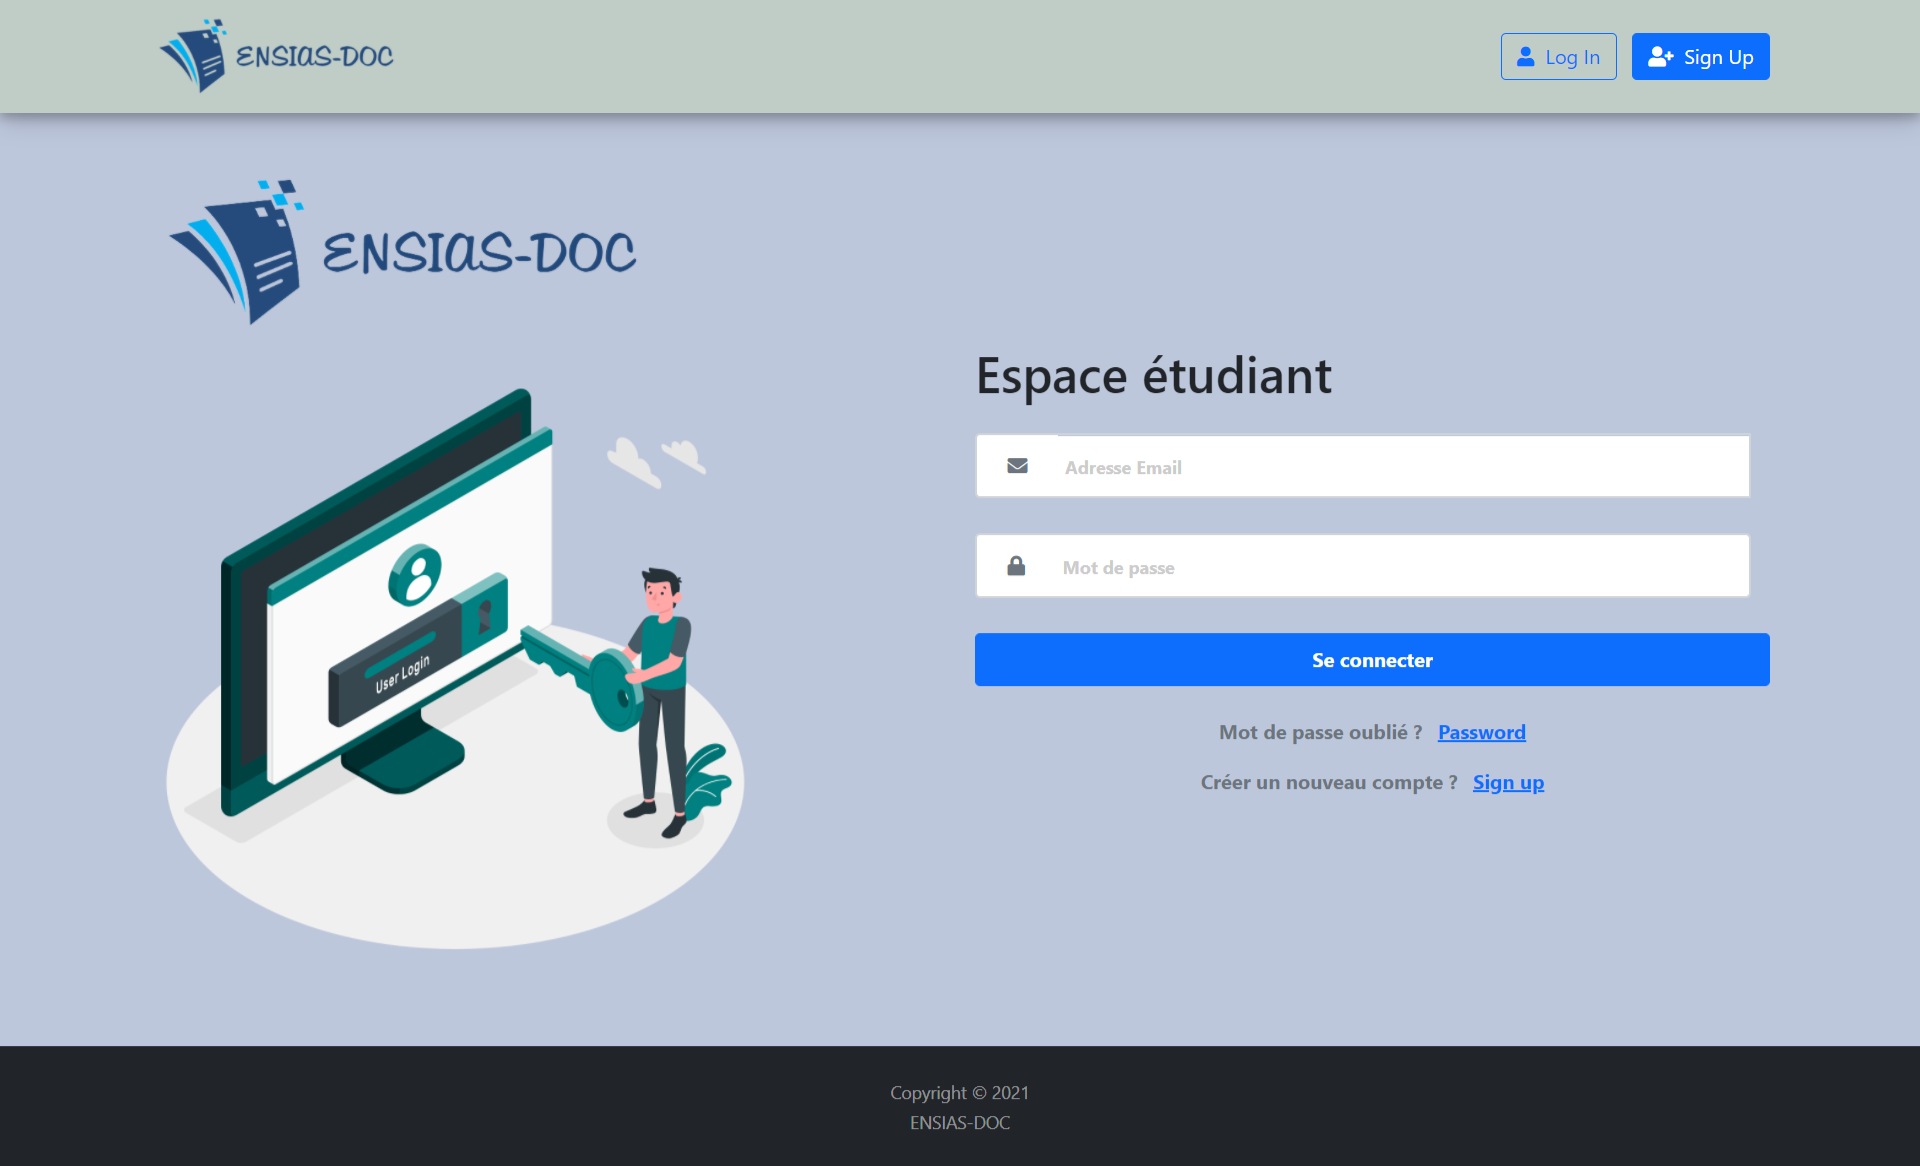
\includegraphics[width=17cm,height=9cm]{login.png}
    \caption{Page d'authentification.}
    \label{Page d'authentification.}
\end{figure}
\subsubsection{Profil}{Le profil contient l'ensemble des informations concernant l'utilisateur inscrit sur l'application y compris: le nom, le prénom, le niveau d'étude, l'adresse mail, le numero de téléphone et la filière.
}
\vspace{1.5cm}

\begin{figure}[H]
    \centering
    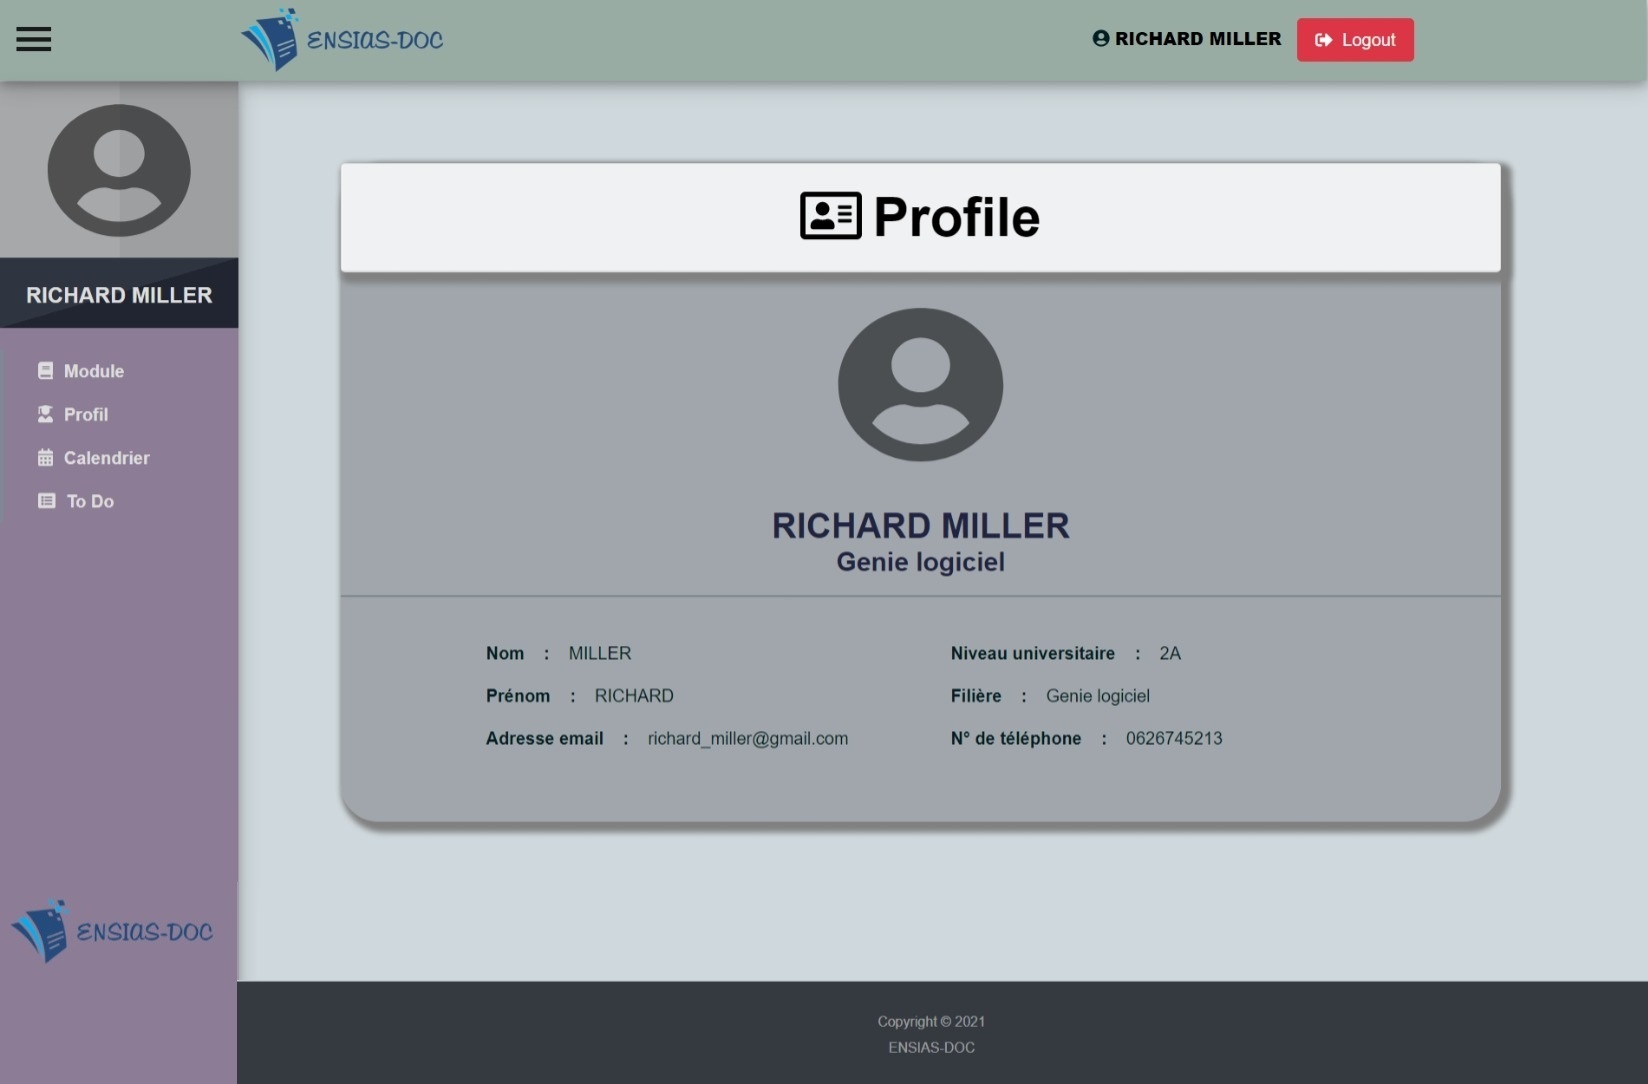
\includegraphics[width=17cm,height=12.5cm]{profil.jpeg}
    \caption{Profil.}
    \label{Profil.}
\end{figure}


\subsubsection{Page de modules}{Cette page affiche l'ensemble des modules que contient l'application et dont l'utilisateur est inscrit, avec une barre de recherhe facilitant la recherche d'un module quelconque.
}
\begin{figure}[H]
    \centering
    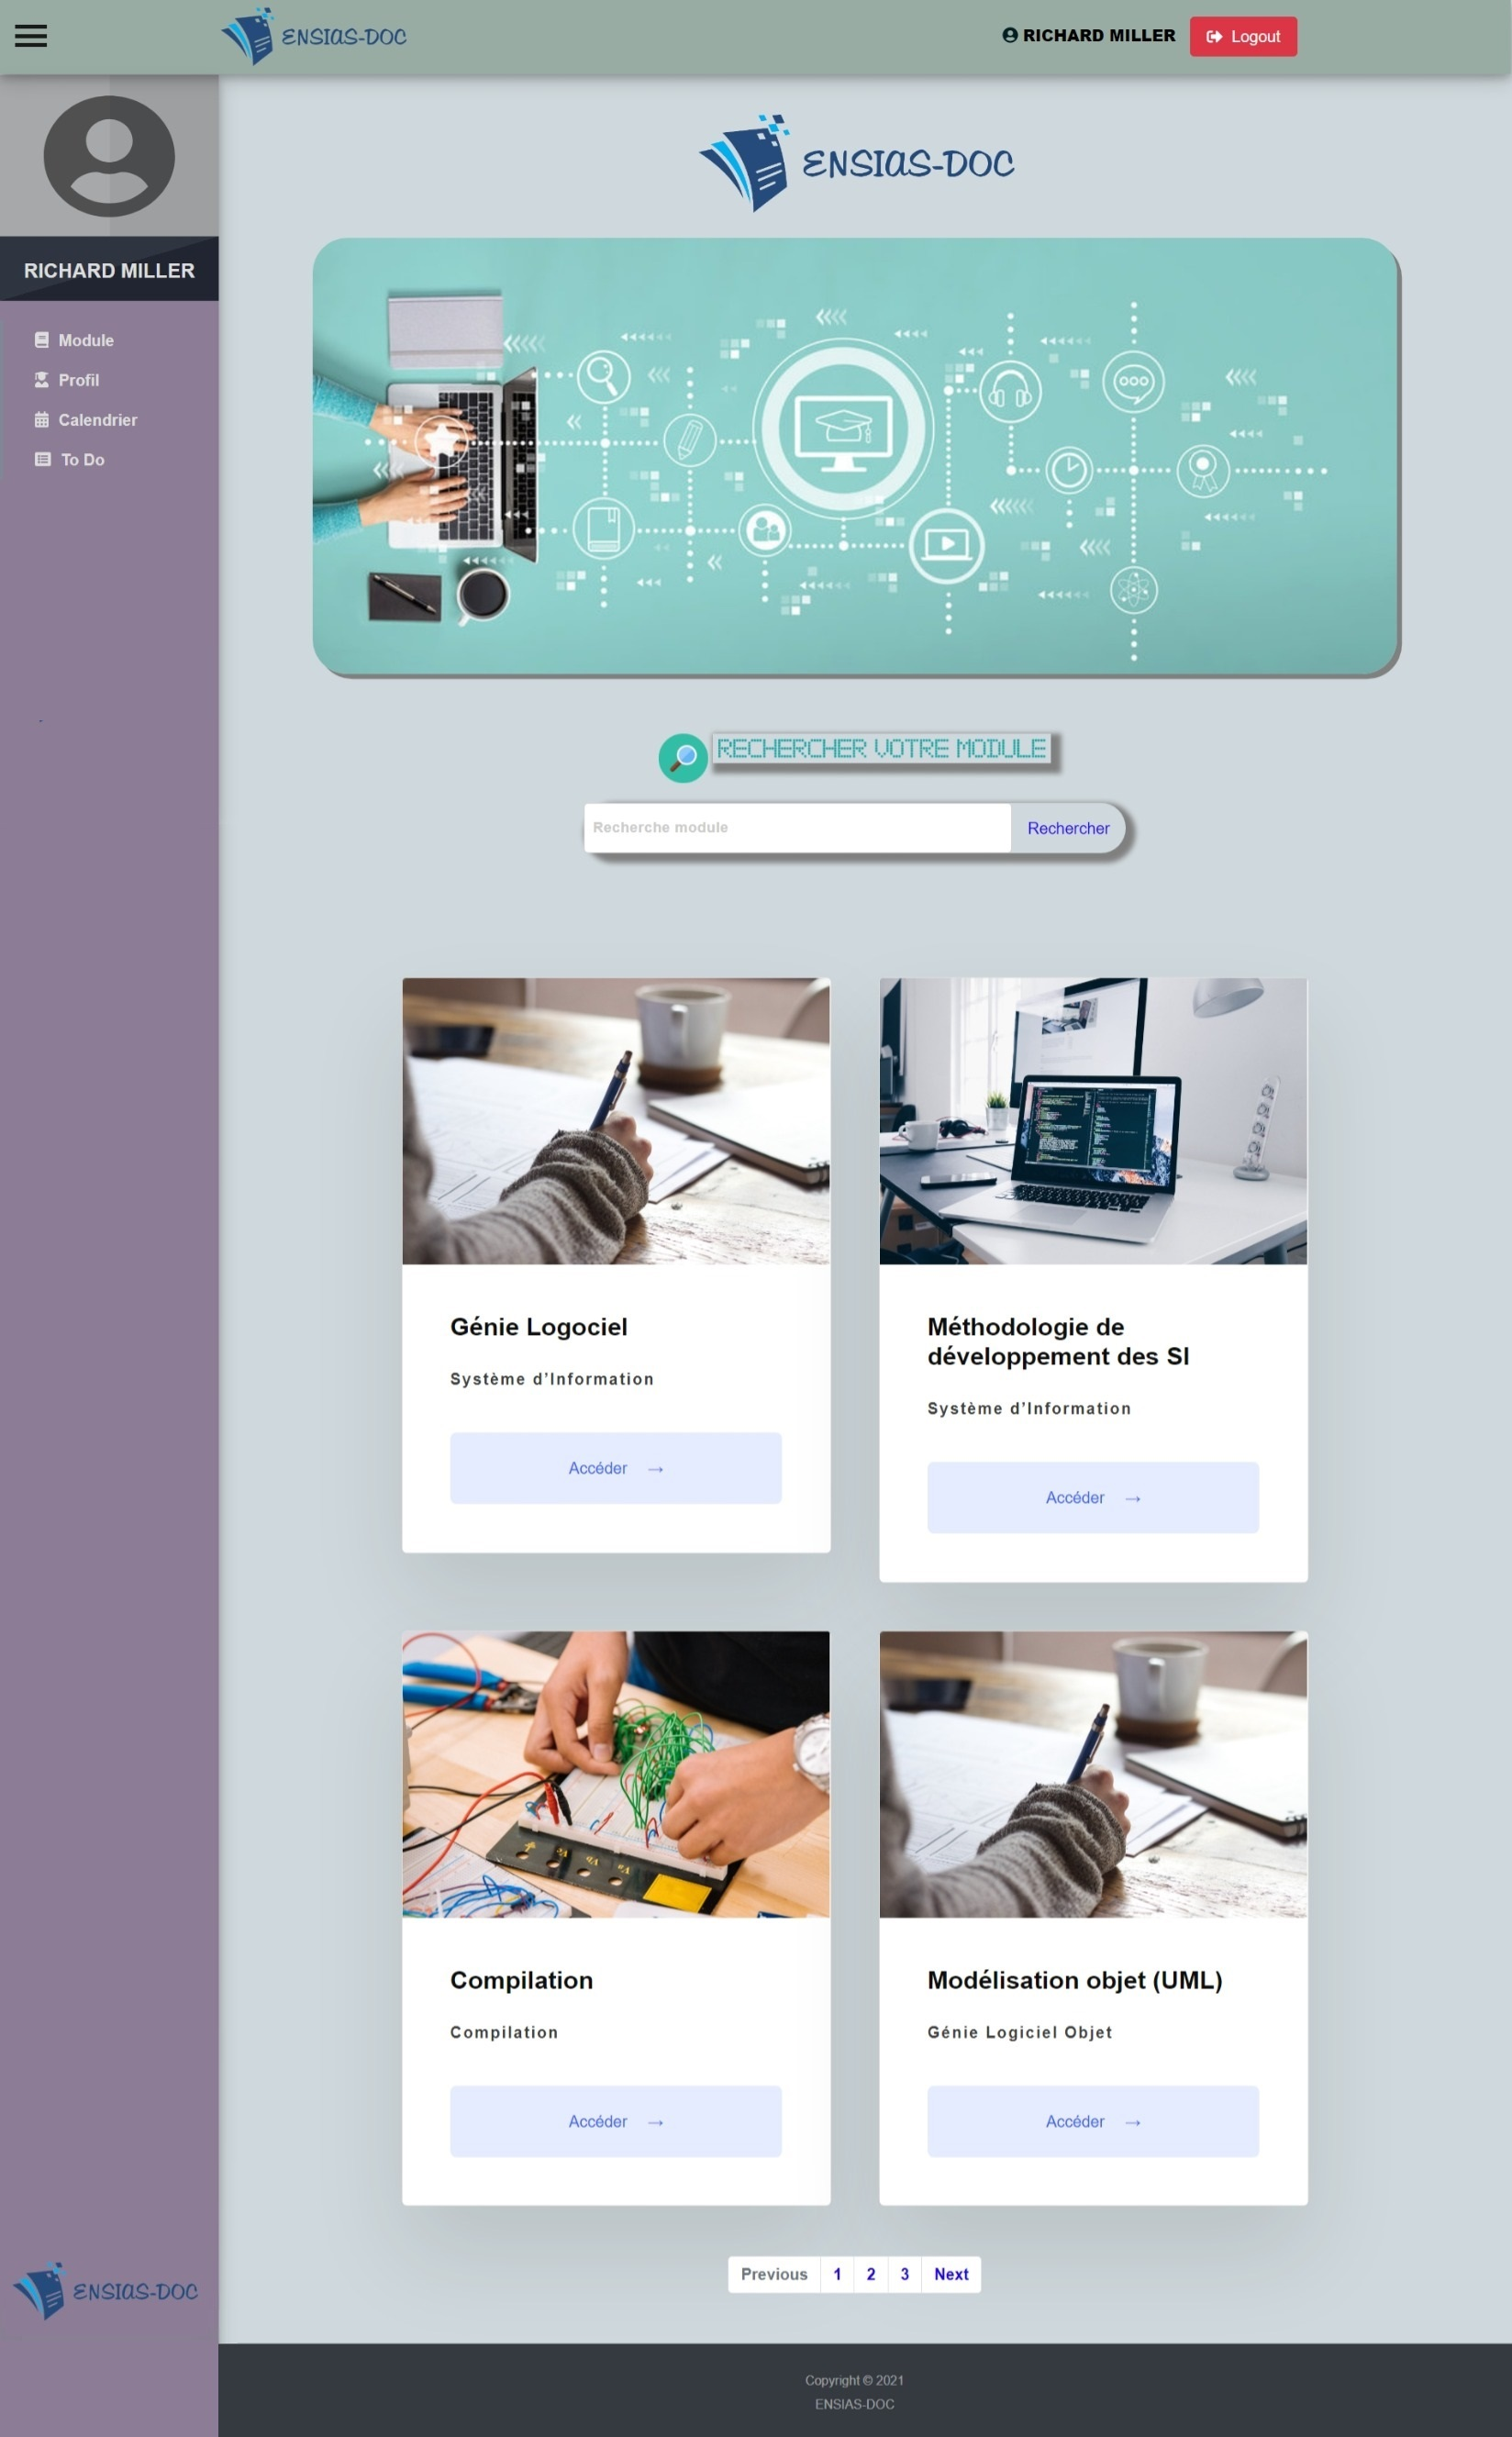
\includegraphics[width=17cm,height=19cm]{module.jpeg}
    \caption{Page de modules.}
    \label{Page de modules.}
\end{figure}

\subsubsection{Page de documents}{Après avoir choisi le module concerné, la liste des document de ce dernier s'affiche. L'utilisateur pourra donc visualiser les documents ou même les téléchrager.
}
\begin{figure}[H]
    \centering
    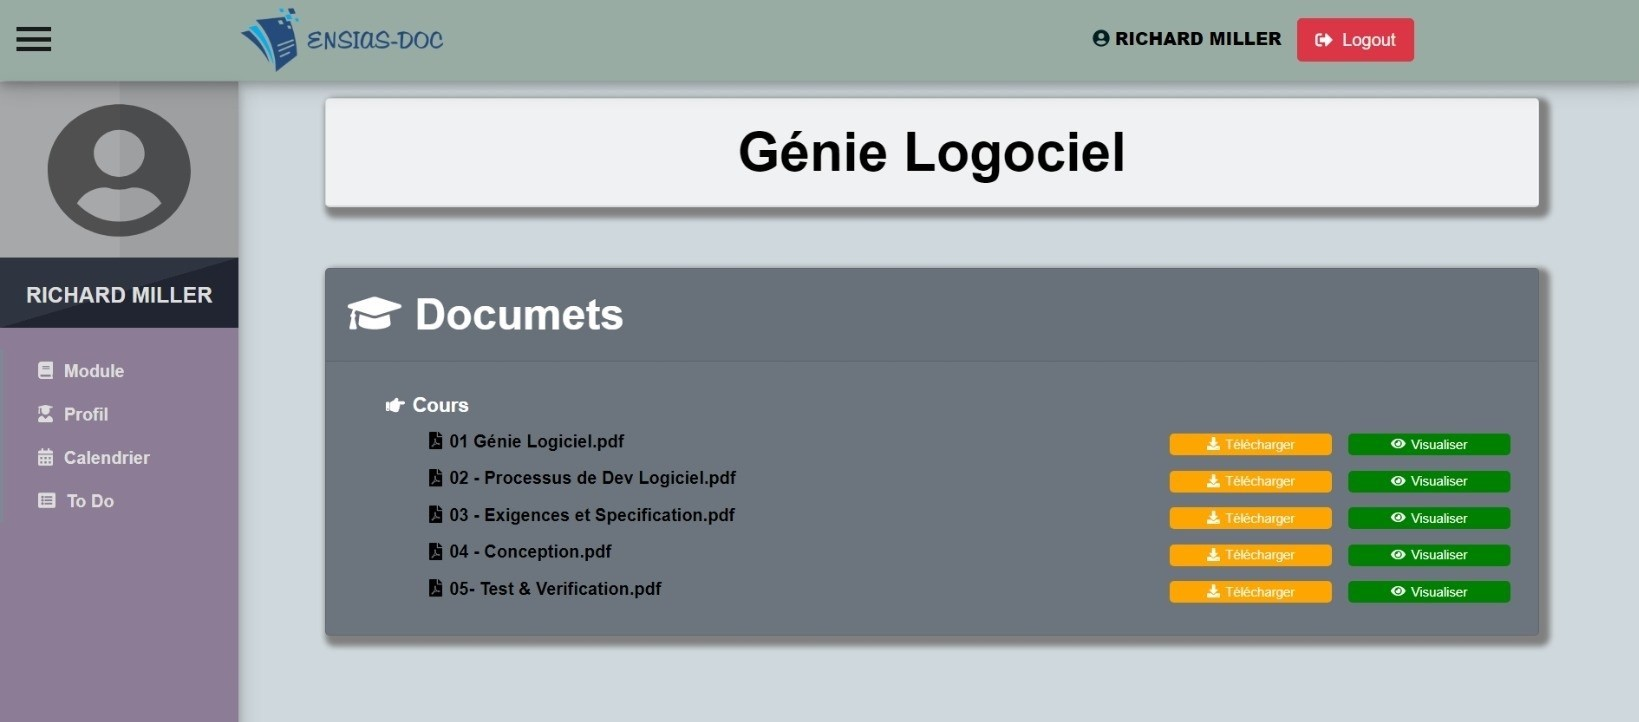
\includegraphics[width=17cm,height=9.5cm]{docc.jpeg}
    \caption{Page de dcouments.}
    \label{Page de documents.}
\end{figure}

\subsubsection{Todo liste }{Chaque utilisateur a sa propre todo liste lui permettant d'ajouter une tache et son délai, la marquer comme terminée, ou la supprimmer. Une alerte s'affiche près des tâches lorsque leurs délais s'approchent d'un jour afin de mieux rappeler l'utilisateur à les achever.
\begin{figure}[H]
    \centering
    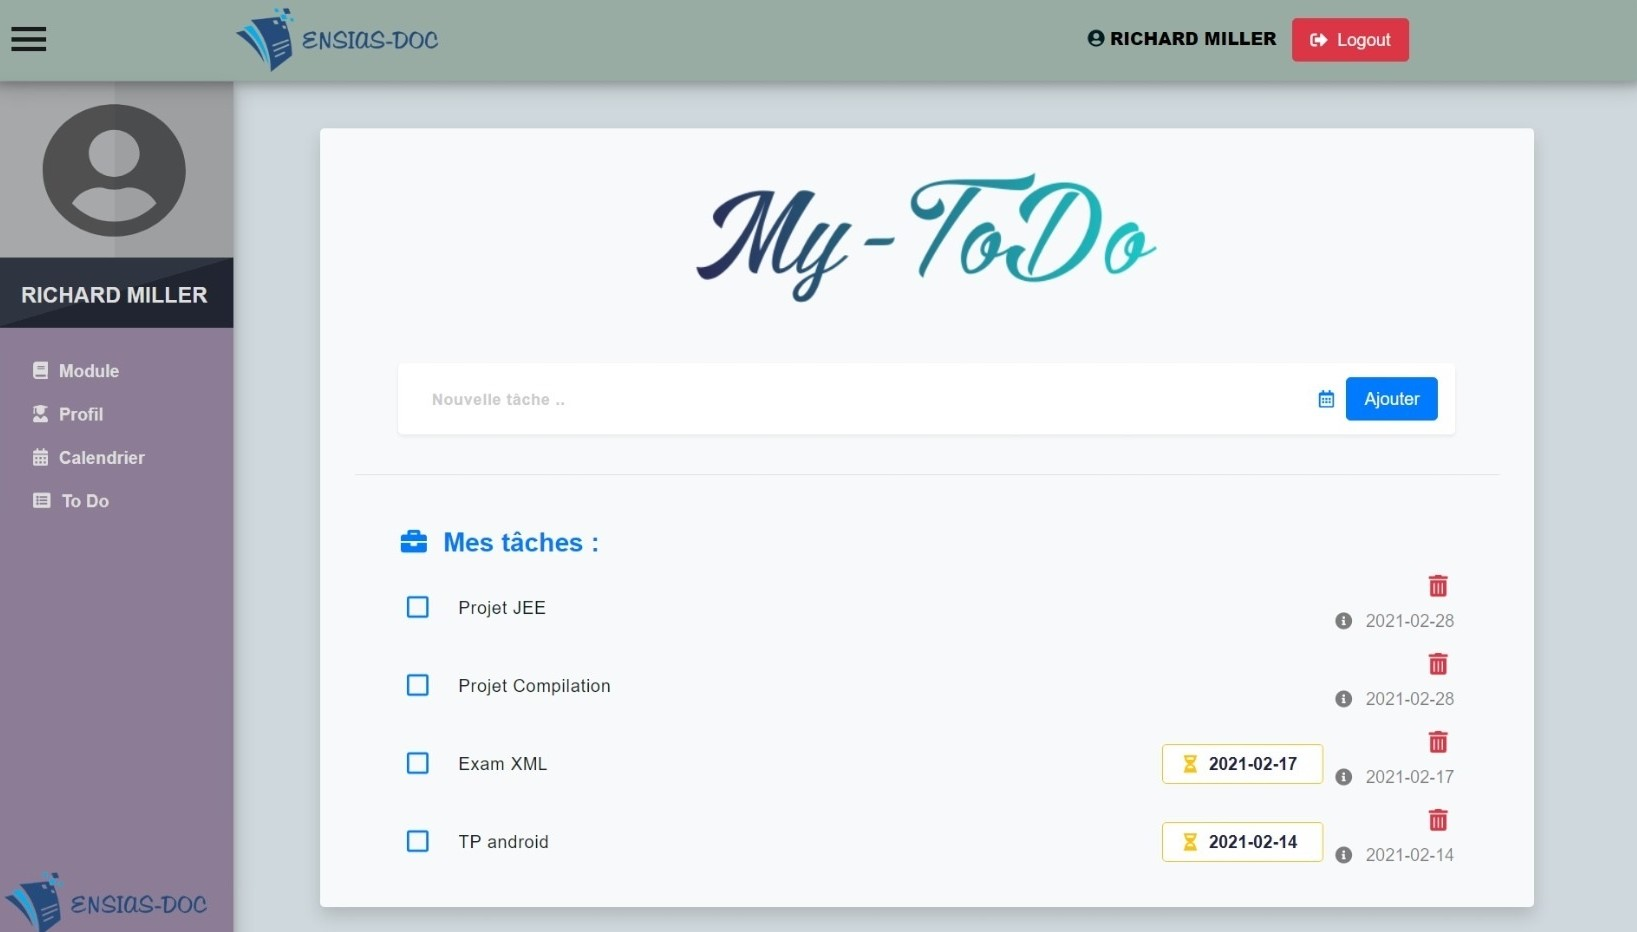
\includegraphics[width=17cm,height=8.5cm]{todooo.jpeg}
    \caption{Todo liste.}
    \label{Todo liste.}
\end{figure}

\subsubsection{Calendrier}{Le calendrier affiche les dates des examens des éléemnt de modules ainsi que toutes les tâches de la todo listes ajoutées par l'utilisateur.
\begin{figure}[H]
    \centering
    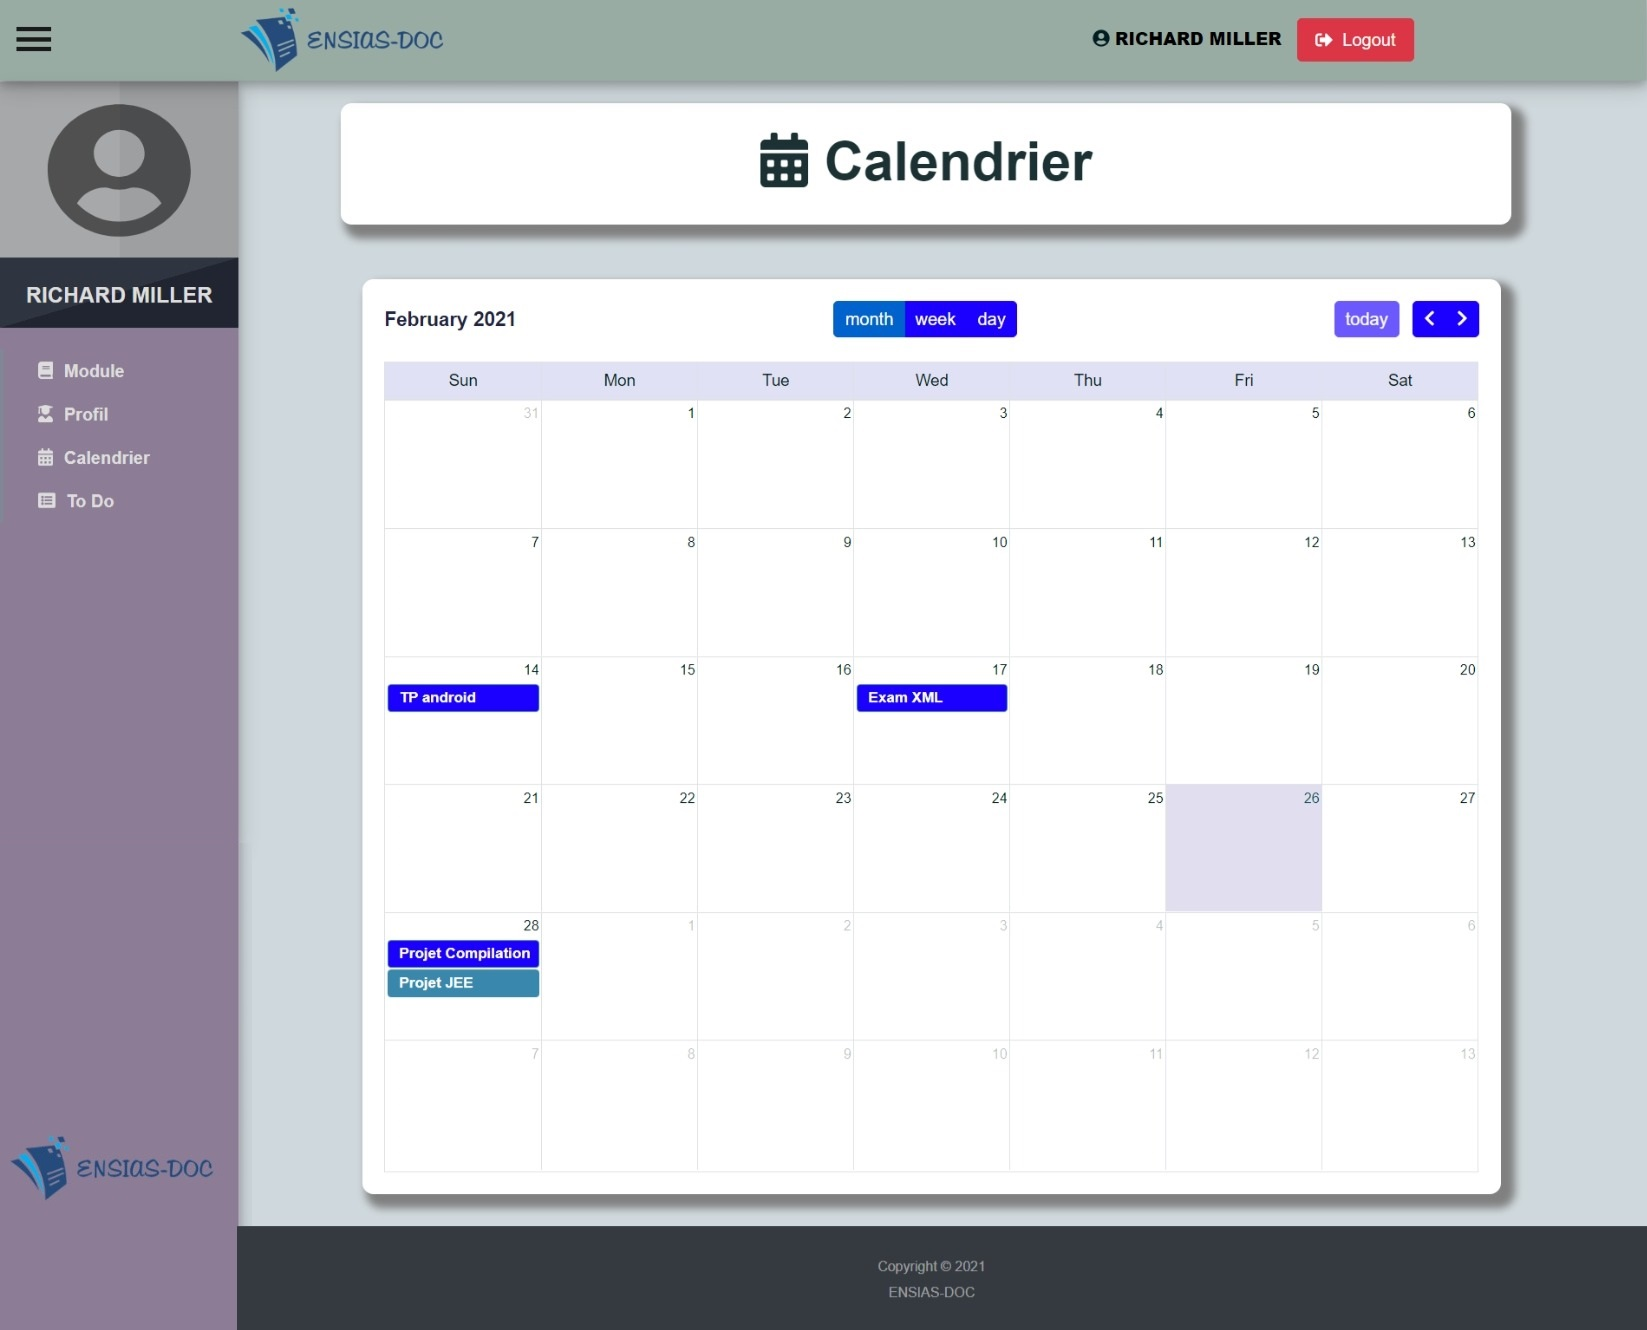
\includegraphics[width=17cm,height=11cm]{calendrier.jpeg}
    \caption{Calendrier.}
    \label{Calendrier.}
\end{figure}

\subsubsection{Espace administrateur}{Cet espace est consacré seulement à l'administrateur de l'application où il a le droit d'ajouter un module, modifier les informations d'un module, ajouter un document à un module déja existant ou ajouter la date d'un exmaen qui s'affichera par la suite aux utilisateurs.
\begin{figure}[H]
    \centering
    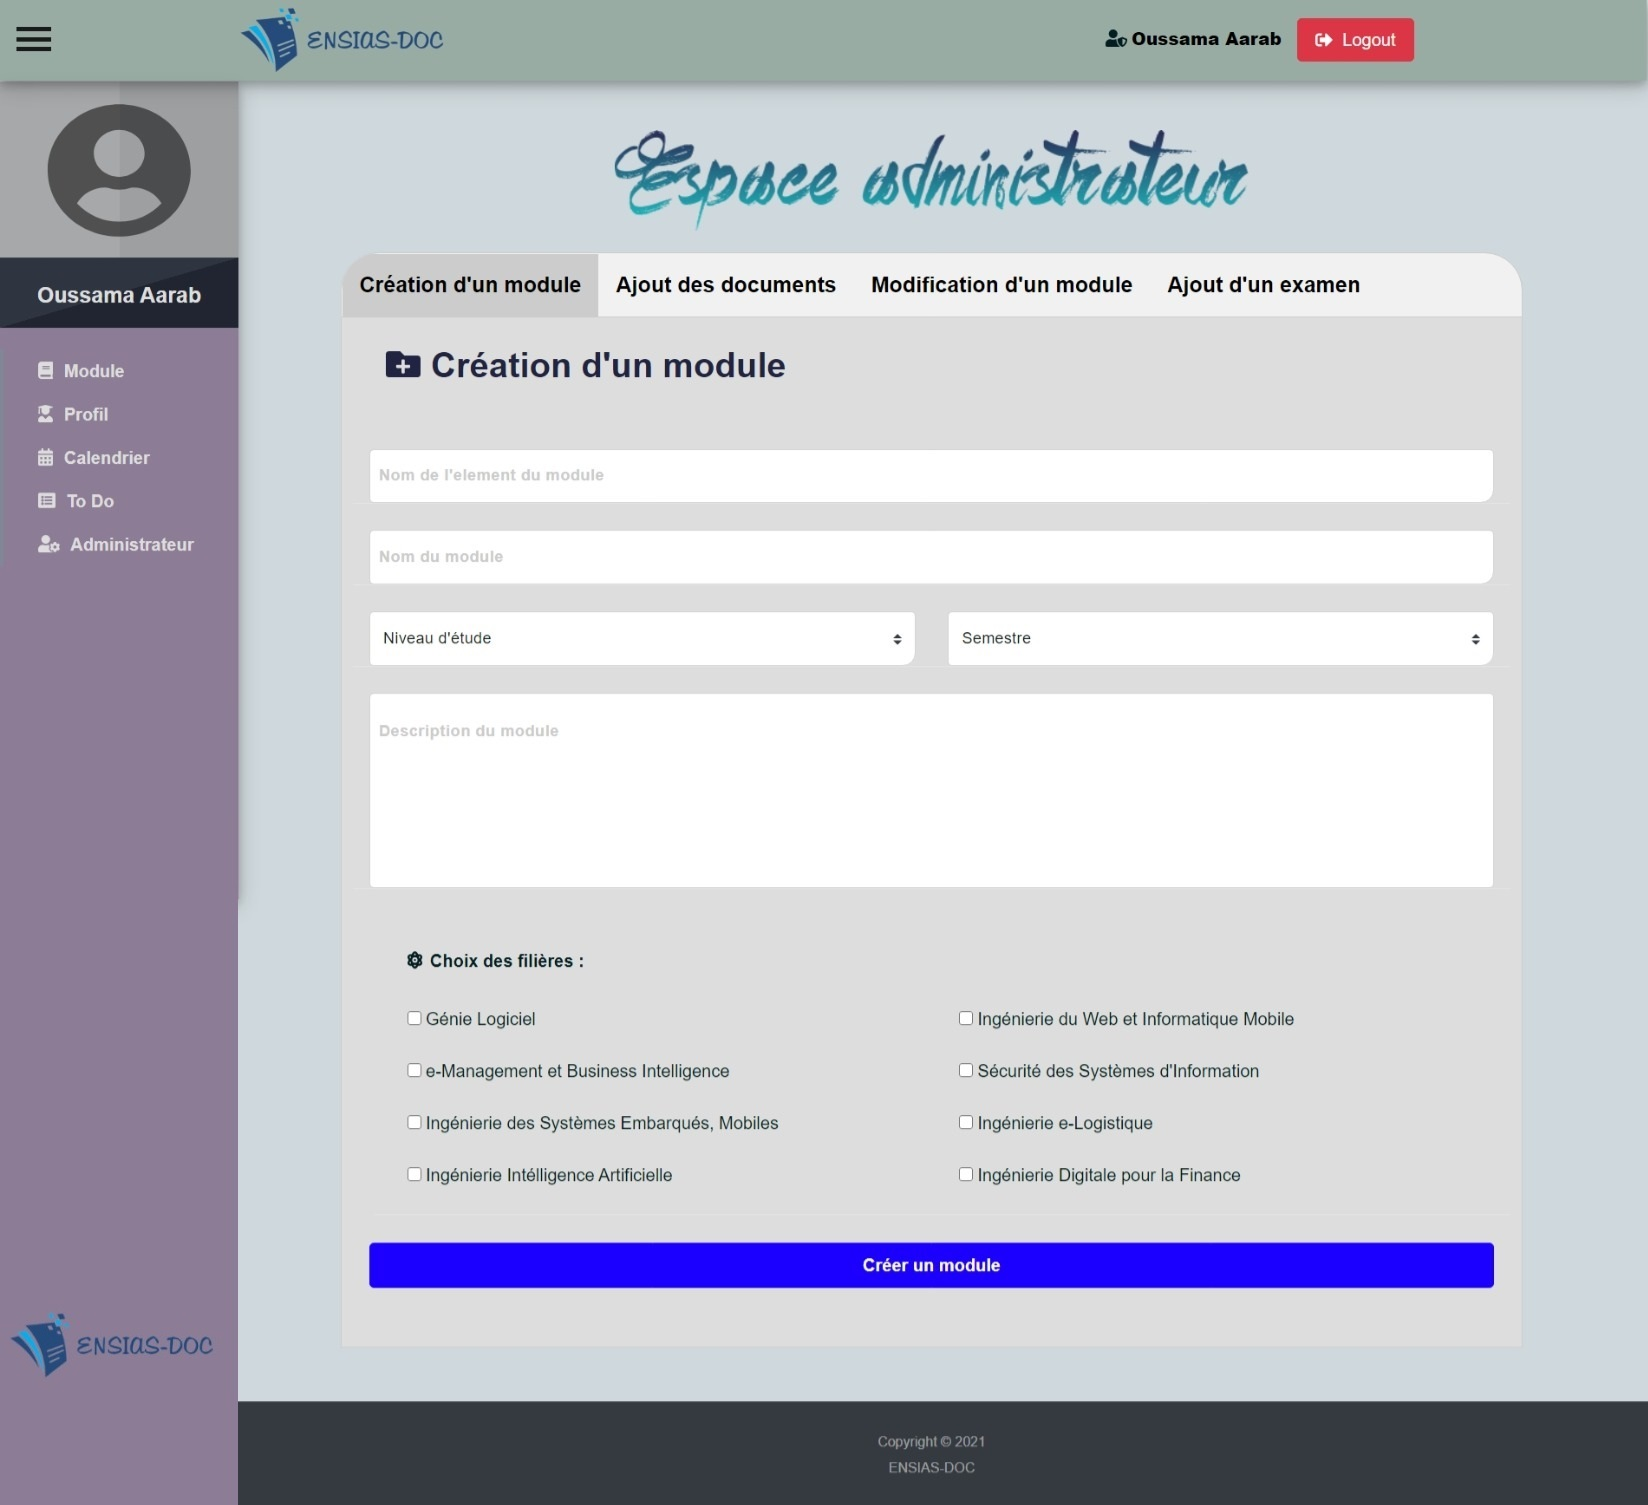
\includegraphics[width=17cm,height=15cm]{Admin.jpeg}
    \caption{Espace admin.}
    \label{Espace admin.}
\end{figure}
\subsection{Conclusion :}
\onehalfspacing\paragraph{}{
Cette partie concerne la réalisation du projet. En effet, nous avons exposé tous nos outils de travail qui nous ont servi pour développer l'application. Nous avons ensuite exhibé nos copies d'écran pour montrer le résultat réel de notre application.

}
\newpage
\begin{center}
    \section*{\huge\textbf{Conclusion générale :}}
\end{center}
\onehalfspacing\paragraph{}{Ce projet consistait en la réalisation d'une application WEB au service des étudiants de l'ENSIAS qui leur assure un espace parfait de révision. Pour ce, il fallait appliquer directement les connaissances acquises en cours : le langage UML[1]
pour modéliser le système de notre application ainsi que celles acquises en cours de l'ingénierie du web pour la phase de l'implémentation. Afin de réaliser un travail aussi important, nous avons fait beaucoup de recherches pour atteindre nos objectifs. Or, notre réalisation
est loin d'être parfaite voir terminée. Nous pensons certes être arrivés à un bon compromis entre réalisme et créativité. Enfin ce projet a été une bonne occasion d'apprendre
de nouveaux outils que ce soit en JEE ou en JSTL. Le projet a été aussi une occasion pour améliorer
notre aptitude pour travailler en groupe.}


%**********************************************%
\newpage
\addcontentsline*{toc}{section}{}
\begin{thebibliography}{20}
\thispagestyle{firstpage}
\onehalfspacing{
\bibitem{}\url{https://netbeans.org/kb/trails/java-ee.html}
\bibitem{}\url{https://mkyong.com/maven/how-to-create-a-web-application-project-with-maven/}
\bibitem{}\url{https://tomcat.apache.org/tomcat-7.0-doc/deployer-howto.html}
\bibitem{}\url{https://netbeans.org/kb/docs/web/mysql-webapp.html}
\bibitem{}\url{https://www.vogella.com/tutorials/JUnit/article.html}
\bibitem{}\url{https://stackify.com/guide-docker-java/}
\bibitem{}\url{ https://getbootstrap.com/, 2014. [Online ; accessed 27-December2018]}
}
\end{thebibliography}
\newpage



\end{document}